\documentclass[12pt,journal,draftcls,letterpaper,onecolumn]{IEEEtran}
\makeatletter
\usepackage{cite}
\usepackage{amssymb}
\usepackage{amsmath}
\usepackage{graphicx}
%\usepackage[retainorgcmds]{IEEEtrantools}
%\usepackage{algorithm}
%\usepackage{algorithmic}
%\usepackage{subfigure}
%\usepackage{url}
\begin{document}
\title{Evolution of Free-riding in P2P Networks}
\author{\IEEEauthorblockN{Heungsik Eom}\\
\IEEEauthorblockA{Electrical and Computer Engineering\\
University of Florida\\
Gainsville, Florida 32611\\
Email: eomhes@gmail.com}\\
\and
\IEEEauthorblockN{P. Oscar Boykin}\\
\IEEEauthorblockA{Electrical and Computer Engineering\\
University of Florida\\
Gainsville, Florida 32611\\
Email: boykin@acis.ufl.edu}
}
\maketitle

\begin{abstract}

Peer-to-peer (P2P) systems rely on cooperation to deliver service. When the
nodes are operated by distinct parties, there may be incentives to benefit 
from the service without contributing to maintain that service. 
Such selfish behavior is called free-riding. It is an open question in P2P systems 
as to when such cooperating systems will collapse in a tragedy-of-the-commons effect
with cooperating users driven from a system due to resources hogging from free-riders.
In this work, we define a simple P2P protocol, and by use of a genetic algorithm, 
show that free-riding naturally evolves when a subset of nodes are allowed to independently 
change the algorithm they follow locally. In the second part of the paper, we show that
by adding tit-for-tat behavior on the part of the majority of nodes, the free-riding subset
will evolve towards a cooperating strategy and will no longer free-ride.
\end{abstract}

\begin{IEEEkeywords}
Peer-to-peer network, Free riders, Genetic algorithm
\end{IEEEkeywords}

\IEEEpeerreviewmaketitle
\section{Introduction}\label{sec:introduction}

Distributed P2P file sharing system has come into the spotlight due to the
ease of organizing and maximizing network ability and scalability.  Without any
centralization, the P2P networks provide service to millions of
users\cite{gnutella,bittorrent}.
Recent studies indicate that over
70 percent of all Internet traffic is due to P2P file sharing system. In spite of the above benefits
and popularity of P2P file sharing systems, there are still many challenges to be handled.
Distributed file sharing systems require each node to work together for good of the
whole network. For that reason, nodes who only take from the network are called free riders.
According to \cite{journals/dsonline/HughesCW05}, P2P
networks are made up of as much as 50 percent free riders who share no files, and
only 25 percent of participants provide for 98
percent of requests from its neighbors.

The question we want to address is the following: do P2P systems require most nodes 
to be altruistic, or can protocols be developed such that even completely
selfish nodes should contribute to the network to maximize their own utility.
Without such protocols, malicious nodes always have an incentive to take,
which reduces quality of service for the altruistic nodes, which in turn flee
due to high cost and limited reward.  Ideally, the optimal local strategy for
a node results in the optimal global strategy such a global utility is
maximized.  This work addresses these research problems.

Firstly, we show that given a simple flooding P2P protocol,
free-riding behavior evolves naturally when a subset of nodes are allowed to
maximize their own utility.  
This results in ``the tragedy of the commons"\cite{tc:tragedy}.

Once we show the natural evolution of free-riders, a second
contribution of this paper is to show that a simple modification
to the flooding protocol can stop the
free-riding behavior.  This is done by penalizing nodes that ignore
query or cache requests.  By adding a tit-for-tat
behavior, the incentive to be a free-rider is removed, which pushes all
nodes to evolve towards a cooperating behavior.

The rest of this paper is organized as follows: In section \ref{sec:system}, We illustrate the network model 
in our simulation and explain how we apply a genetic algorithm to find optimal
node behaviors. In Section \ref{sec:evolution}, 
we show the natural evolution of free riders.  Section
\ref{sec:countermeasure} gives a modified protocol which removes the
incentive to free-ride and we see that nodes evolve to contribute, and
not free-ride.
Prior works about the use of a genetic algorithms on P2P network and the
problem of free-riding are reviewed in Section \ref{sec:related}. Lastly,
conclusion and future work are presented in Section \ref{sec:concl}.

\section{System Description}\label{sec:system}

For our simulation, we model an unstructured P2P network for file
sharing\cite{journals/comsur/LuaCPSL05}. In unstructured P2P file sharing, all the nodes
equally act as both roles of servers and clients.  In our model there is no
locality for nodes and contents such as DHT, so implementing the network is
very simple.  We define a very simple P2P protocol which is very similar to
the original Gnutella protocol.  Message broadcasts are done by sending a
message with a $TTL$.  Upon receiving a message, each node decrements the
message $TTL$ and if the $TTL$ is greater than zero the node forwards that message
to each neighbor other than the one from which the message was received.  To
share objects, a node broadcasts a cache message and to query for objects a
node sends a query message.  Each node follows its own version of the protocol
defined by certain fixed parameters:

\begin{itemize}
\item {\bf Time To Live ($TTL$):} the number of hops each query and cache message takes
before expiring.
\item {\bf Connection Limit ($L_C$):}
the maximum number of neighbors each node will accept.
\item {\bf Message ignore probability ($p_i$):}
the probability that a caching of querying 
\end{itemize}

Each node is initialized with values for the above parameters.  Subsequently,
we evaluate the performance of this network for each node.  We evaluate the
costs and benefits each node experiences which is combined into node fitness.
We operate a genetic algorithm (GA)\cite{genetic} on the sets of nodes using
the fitness we obtain from the network simulation, and we assume that each
node will individually evolve towards a higher local fitness, \emph{not
towards a global notion of fitness}.  It is worth repeating that nodes are not
trying to optimize the common global network fitness, but they are only
seeking to optimize \emph{their own fitness value}.

To build a system complex enough to see a rich behavior, we create two
``species" or groups of nodes.  One is defined to be 10\% of the total
population, and the other accounts for 90\%.  In our simulations, network size
was 90: 81 in the big group and 9 in the small group.
Mating only happens in the same group: both of parents, father and mother,
need to be from the same group.  The intuition is that even
completely selfish behavior on the part of the smaller population should not
destroy the entire network performance.
Figure \ref{fig:simblock} shows the block diagram for our simulator.

\begin{figure}
\centering
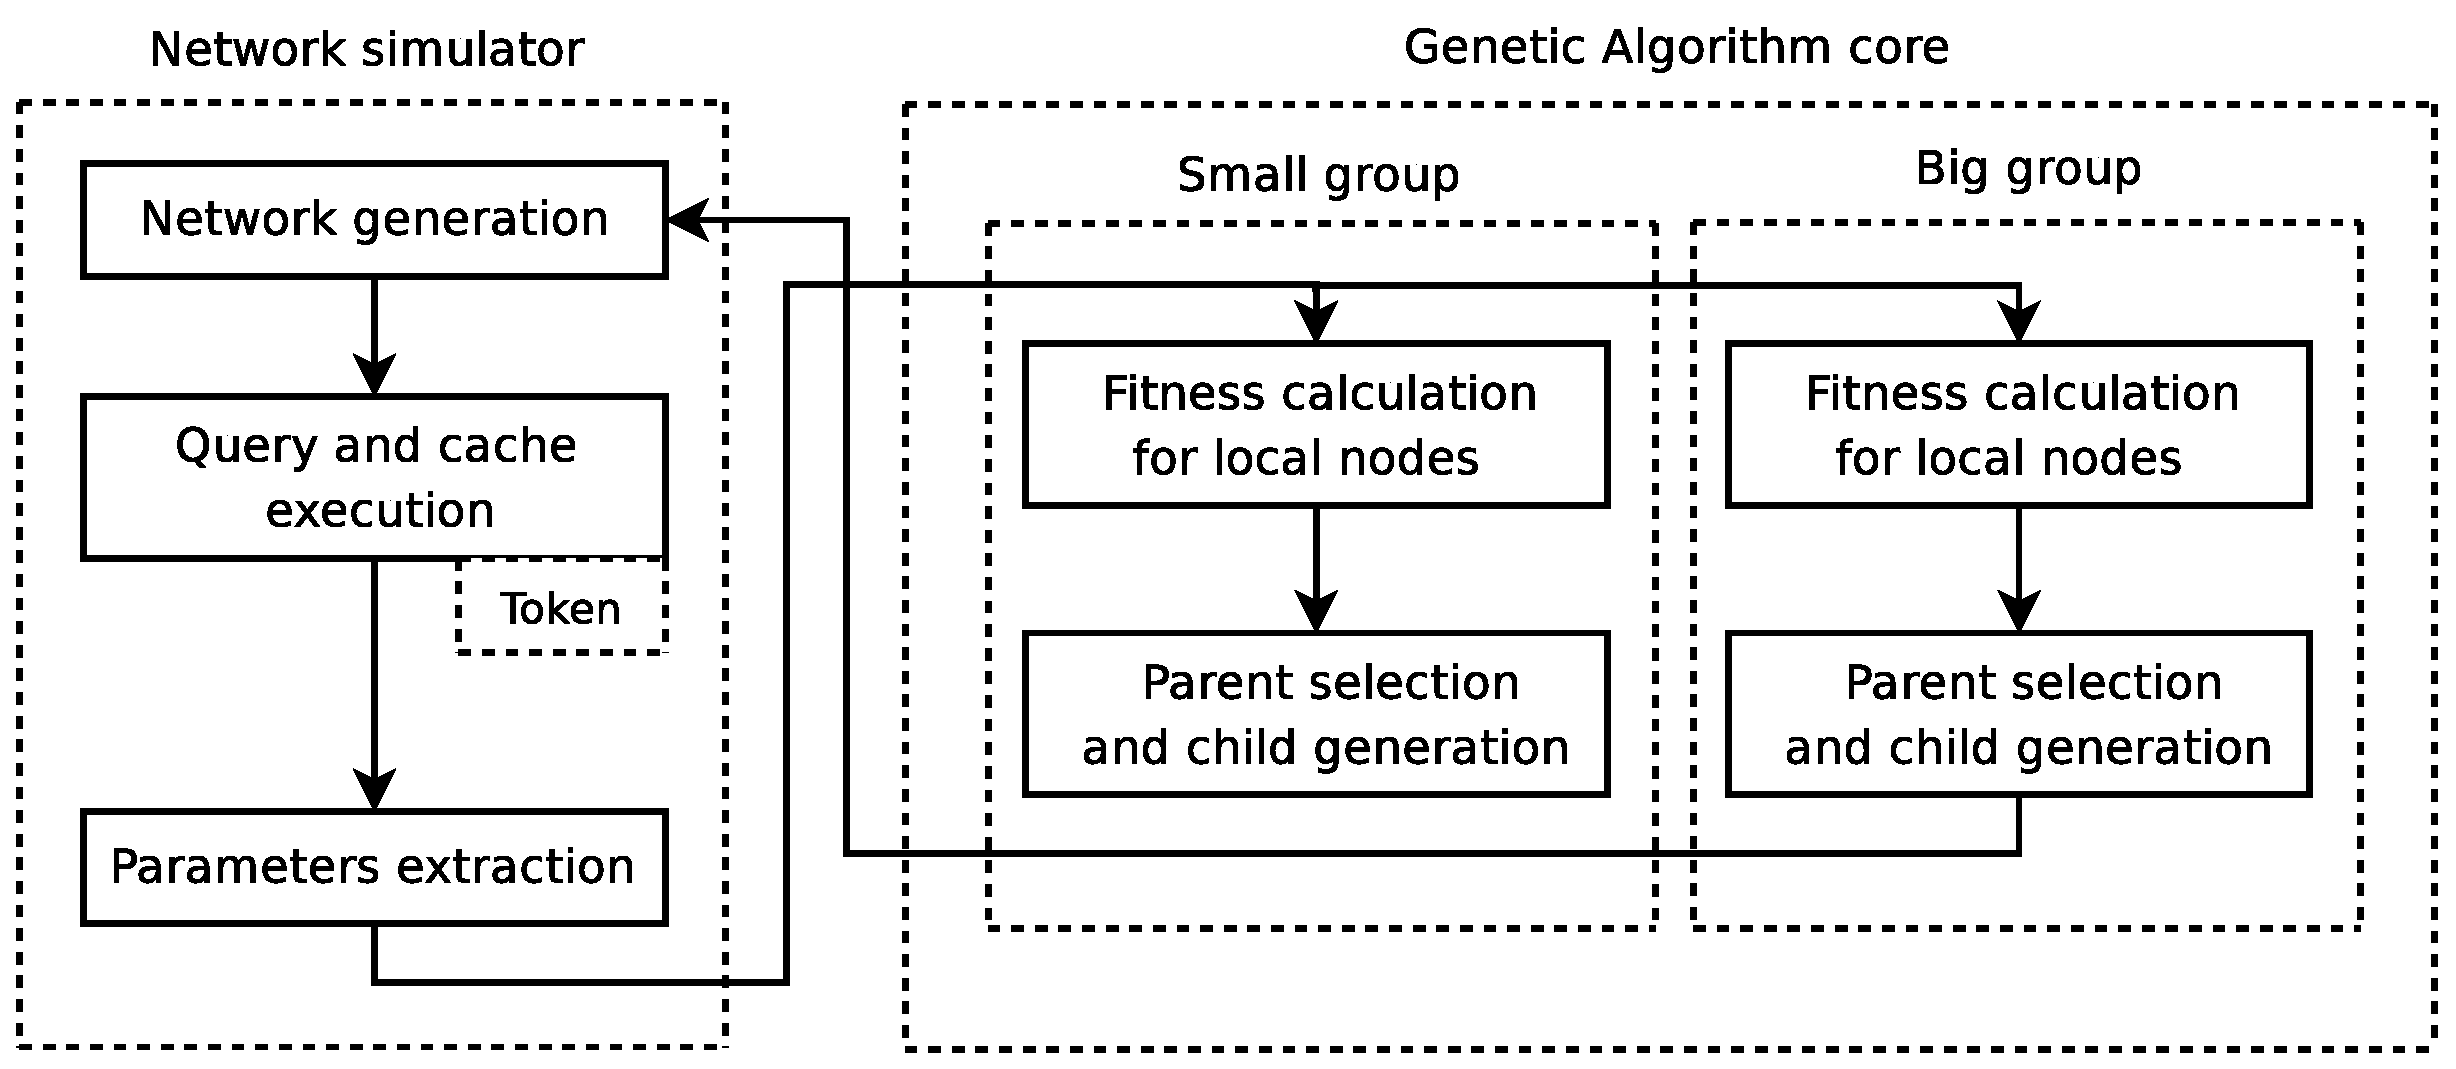
\includegraphics[width=5.2in]{simblock}
\caption{Block diagram for the simulator.  Network simulation determines fitness values,
the genetic algorithm uses fitness values, parent selection and cross-over to produce the next
generation of nodes, then we return to the network simulator and repeat.} 
\label{fig:simblock}
\end{figure}

\subsection{Network Modeling}\label{sec:netmodel}
Figure \ref{fig:network} shows our model for the unstructured p2p network for file sharing with
$N$ nodes. To construct the network model, we use \emph{Netmodeler} which is a C++ library for
modeling networks developed at University of Florida and UCLA\cite{netmodeler}.

\begin{figure}
\centering
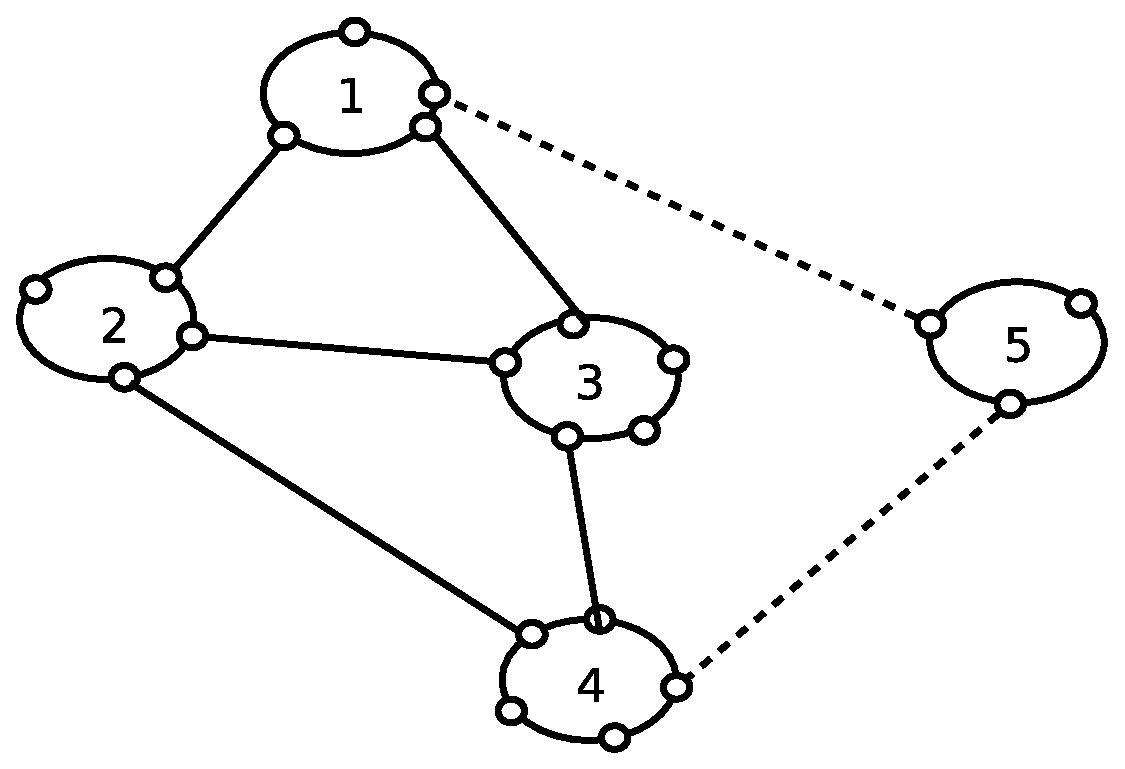
\includegraphics[width=2.5in]{network}
\caption{Example network of five nodes.  Small circles represent available connections
for each node, lines represent connections.} 
\label{fig:network}
\end{figure}

Our network modeling consists of two phases; network configuration and network operation.
The network configuration phase creates a random network with the constraint
that each node does not have more than its allowed number of neighbors.
In the first generation of the genetic algorithm,
each node's $TTL$ and $L_C$ are assigned randomly from a uniform distribution.
In Figure \ref{fig:network},
circles around the nodes represent $L_C$.
Message ignore probability reflects the
selfishness of users. In other words, nodes which have a high message ignore
probability, seldom respond to query and cache actions from its neighbors and
don't route messages needed to give other nodes a high hit-rate.
In the first generation, message ignore
probability is also assigned to each node randomly from a uniform distribution.

After the network configuration is completed, each node executes cache and query actions as
follows: The node $n_A$ creates a randomly generated
character string $I_A$ as an item to share.
This string models data and may represent an entire shared object or metadata about an object
that $n_A$ wishes to share.
In our protocol, the node $n_A$ sends a cache message to replicate its own
item to neighbors with a broadcast whose depth depends on the value of $n_A$'s
$TTL$.  This is repeated for each node.  After all nodes have cached their
content, we begin the querying.  When querying, node $n_A$ sends a query
message that would match one randomly selected item $I_r$.  A broadcast query
message is sent to all neighbors with the node's own $TTL$.  This process is
repeated with a randomly selected query 100 times for each node to estimate
the node's hit-rate. The hit-rate for each node is estimated in the same way.

Query hits are the only benefit a node gets from the network.  In addition to
measuring the benefits, we also measure the costs: network bandwidth,
storage space, and CPU time.
For each node, hit-rate, CPU and disk cost are defined by
\[
Hitrate=\frac{Query_{resp}}{Query_{req}}
\]
\[
CPU\_cost=Message_{recv}+Message_{proc} \times N_{items}
\]
\[
disk\_cost=N_{items}
\]

where $Query_{req}$ and $Query_{resp}$ refer to the number of queries that 
the node requests and responses received respectively. $Message_{recv}$ and $Message_{proc}$ 
represent the number of messages that the node received and processed. 
$N_{items}$ is the number of items that the node stores.  Each incoming message, 
query and cache message, increases $Message_{recv}$ and $Message_{proc}$, 
and with probability $P_i$ is ignored.  If it is not ignored, we process the message 
and increase $Message_{proc}$.  Particularly, if cache message is accepted, 
$N_{item}$ also increases by 1. Note that by ignoring messages, a node can reduce 
the number of messages it has to process, but not directly the number it receives.  Also by ignore cache
requests, a node does not need to increase $N_{items}$.  Clearly, increasing
the probability of ignoring messages would seem to reduce costs.

\subsection{Genetic Algorithm}\label{sec:genetic}
We assume that nodes will want to increase their benefit and reduce their
costs.  As such, the strategy of ignoring some messages may 
arise naturally.  We define a fitness for each node which is increasing in the
benefits and decreasing in the costs:
\[
Fitness = \exp\left(\alpha_{h}\times hitrate-(\alpha_{c}\times cpu_{cost} +
\alpha_{d}\times disk_{cost})\right)
\] where $\alpha_h, \alpha_c, \alpha_d$ represent weighting factors.
Note that the fitness function has positive and
negative parts.
The positive part includes the hit-rate and negative part consists of the CPU and disk
cost. Therefore, as CPU and disk cost decrease and hit-rate increases, fitness will increase.

We apply a genetic algorithm (GA) to optimize each node's local fitness.  Note, we
are not fixing one strategy for all nodes and optimizing the network's
fitness, but each node should find a maximum fitness such that it will only
reduce its fitness by changing it's local parameters of $TTL$, $L_C$
and $p_i$.
We use a standard genetic algorithm where
each node in the network is regarded as individual, and 
node characteristic parameters -- $TTL$, $L_C$ and $p_i$-- are
considered as the genes for each individual.

After each network operation phase, each node estimates its own hit-rate, CPU and disk cost and
the GA core calculates the fitness of each node. The fitness function is used to
rank nodes for parent selection. Based on the ranked nodes, GA core selects parent nodes and
generates child nodes by crossover and mutation operation of three genes of parents ;
$TTL$, $L_C$, and $p_i$. The crossover is defined as:

\begin{itemize}
\item{\bf $TTL$ -}
$Random[Father, Mother]$
\item{\bf $L_C$ -}
$Random[Father, Mother]$
\item{\bf $p_i$ -}
$Average[Father, Mother]$
\end{itemize}
For the integer parameters, $TTL$ and $L_C$, we choose uniformly 
over the region given by the father and mother values.
For the real parameter $p_i$, we average the mother
and father value.  After crossover, we apply mutation.  For the integer
parameters, with some probability we randomly increase or decrease the value
by one.  For the real parameter we choose a new value uniformly from the
region which is $m\%$ as large as the parameter value.  For instance, if the
parameter was $p$ we would select uniformly from the region $[p(1-m/2),
p(1+m/2)]$.

For our simulation, we set 0.1\%, 0.1\% and $5\%$ for mutation of $TTL$, $L_C$
and $p_i$ respectively. Because the values of $TTL$ and connection limit are
positive integers and bigger than message ignore probability, we set relatively small value for
the mutation of $TTL$ and connection limit over message ignore probability. In
the parent selection
process, we have tried several methods to reduce the computation load of
executing genetic algorithm.  The selection method we used which gave the best
convergence to a maximal fitness value was
the square-root selection method: at each time step, we rank the fitness values
from most to least fit.  Then we compute $N_s = \lceil\sqrt{N}\rceil$, and prepare
following children in order: Child(1, 1), Child(1, 2),$\ldots$, Child(1, $N_s$),
Child(2, 2), Child(2, 3), $\ldots$ Child(2, 1 + $N_s$), Child(3,3), $\ldots$, where
Child($i$,$j$) is a child of node $i$ and $j$ according to our above mating rules.
From
this ordered set of children we select the first $N$ children.  This guarantees
that even with a small population, the top $\sqrt{N}$ individuals have children
that make it into the next generation.
Finally, we observed that allowing any two nodes to mate created a single
species of node and prevented any nodes from evolving too far away from the
average behavior.  To more accurately model nodes which may radically depart
from the average behavior we created two populations, the big group and small
group. Mating only happens in the same group: both of parents, father and mother, need to be
from the same group. In our setting, the ratio of small group and big group is 1 to 9.

\section{Evolution of free-riders}\label{sec:evolution}

For our simple protocol, we consider nodes with a high value for $p_i$ to be
free-riders.  These nodes make queries, but seldom handle cache or query
messages.  Put another way, they consume network resources when others process
their queries, but they don't use their resources to serve others.

For a given node, in a single generation, increasing $p_i$ will decrease its
costs, but not change its hit-rate.  Figures
\ref{fig:nocpucost}-\ref{fig:fitness1} demonstrate the point that for a fixed
node, increasing $p_i$ decreases costs without directly effecting hit-rate.
This is because
the nodes which have high $p_i$ process fewer cache and query
messages, they have smaller CPU and disk cost than low $p_i$ nodes. However, in
figure \ref{fig:nohitrate}, it is shown that the distribution of hit rate is unrelated to message ignore
probability.
Putting it together, as shown in Figure \ref{fig:fitness1}, the fitness tends
to increase with higher values of $p_i$.

\begin{figure*}
\begin{tabular}{c c}
\begin{minipage}[t]{3in}
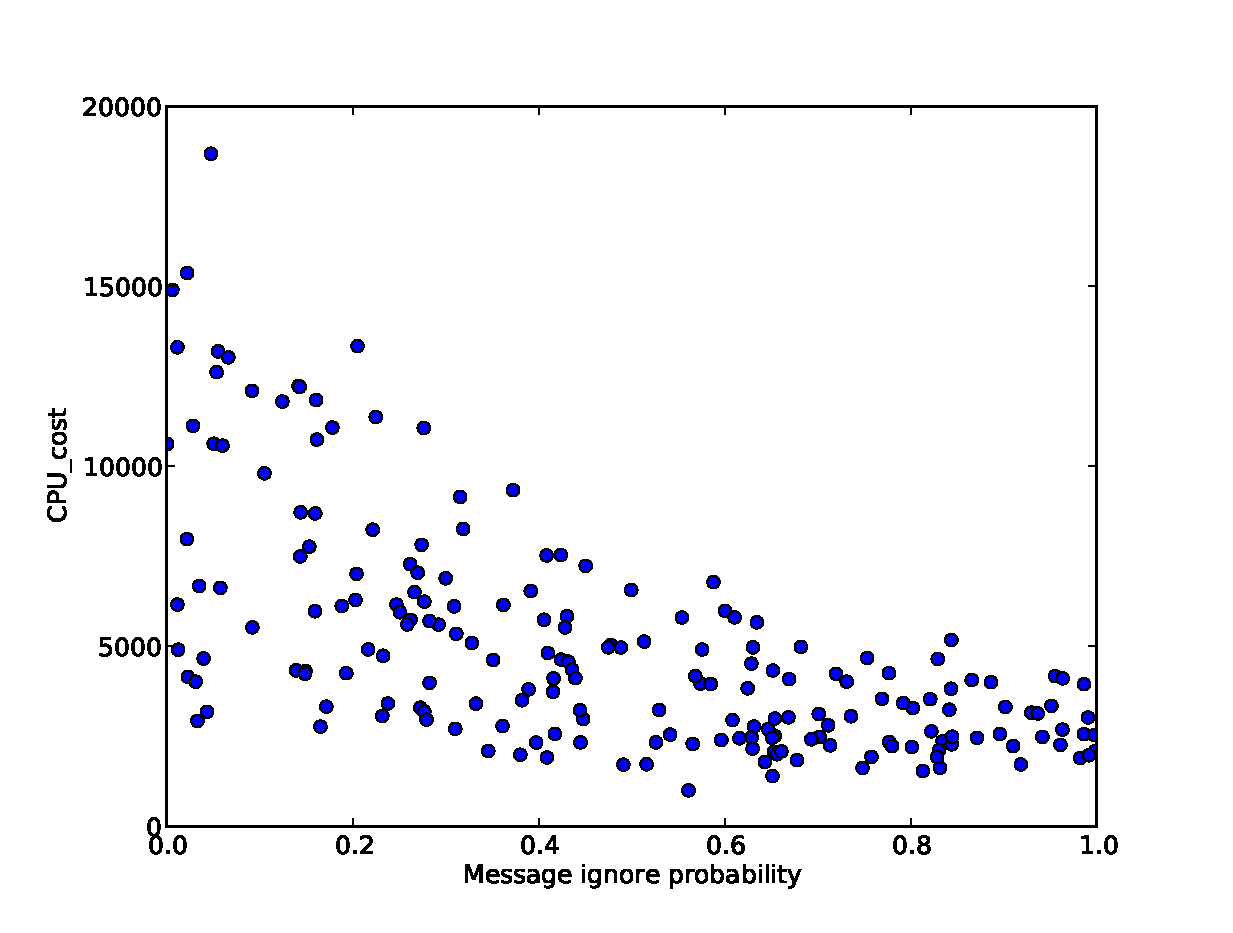
\includegraphics[width=3in]{cpucost1}
\caption{CPU\_cost for message ignore probability}
\label{fig:nocpucost}
\end{minipage}
\begin{minipage}[t]{3in}
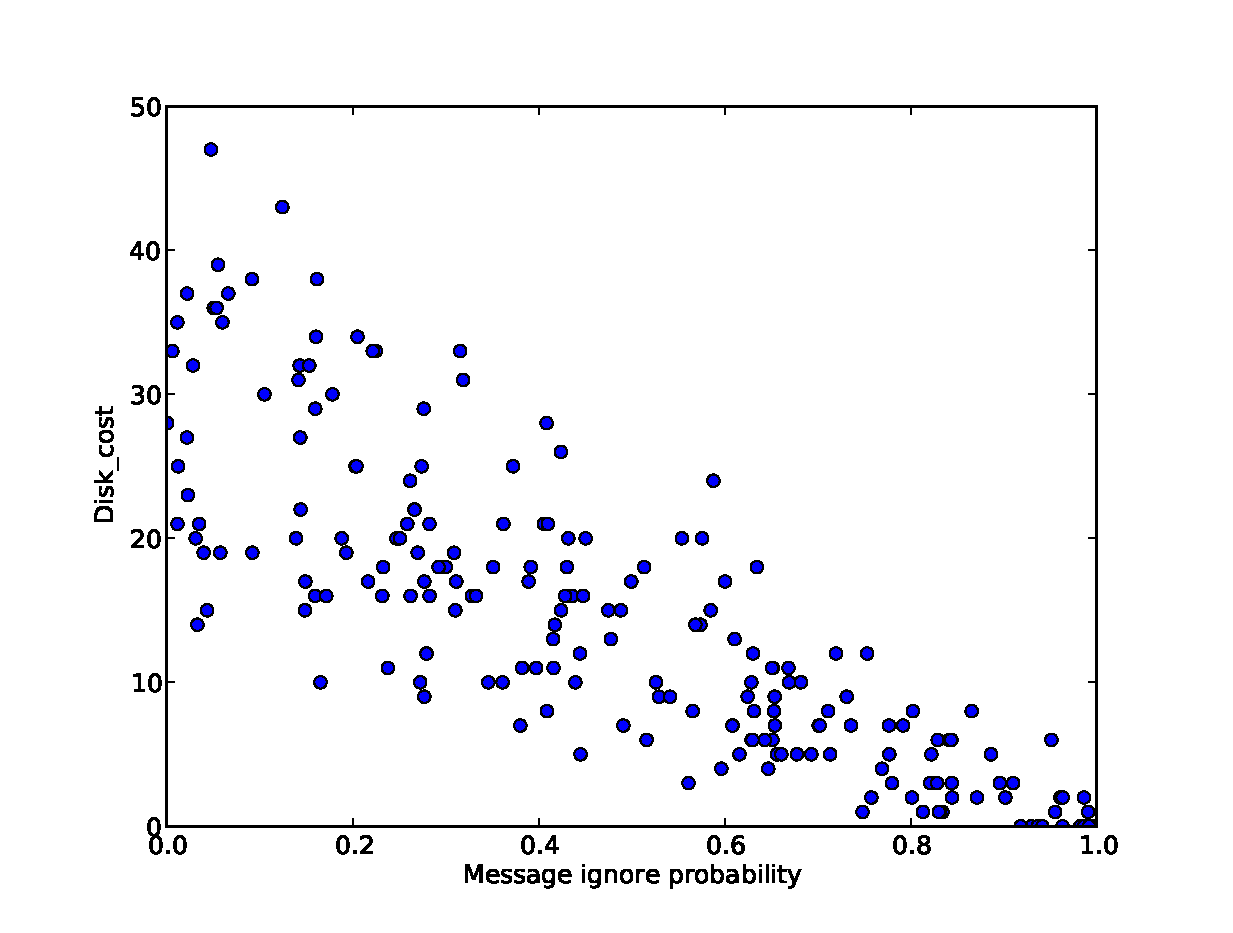
\includegraphics[width=3in]{diskcost1}
\caption{Disk\_cost for message ignore probability}
\label{fig:nodiskcost}
\end{minipage}
\end{tabular}
\end{figure*}

\begin{figure*}
\begin{tabular}{c c}
\begin{minipage}[t]{3in}
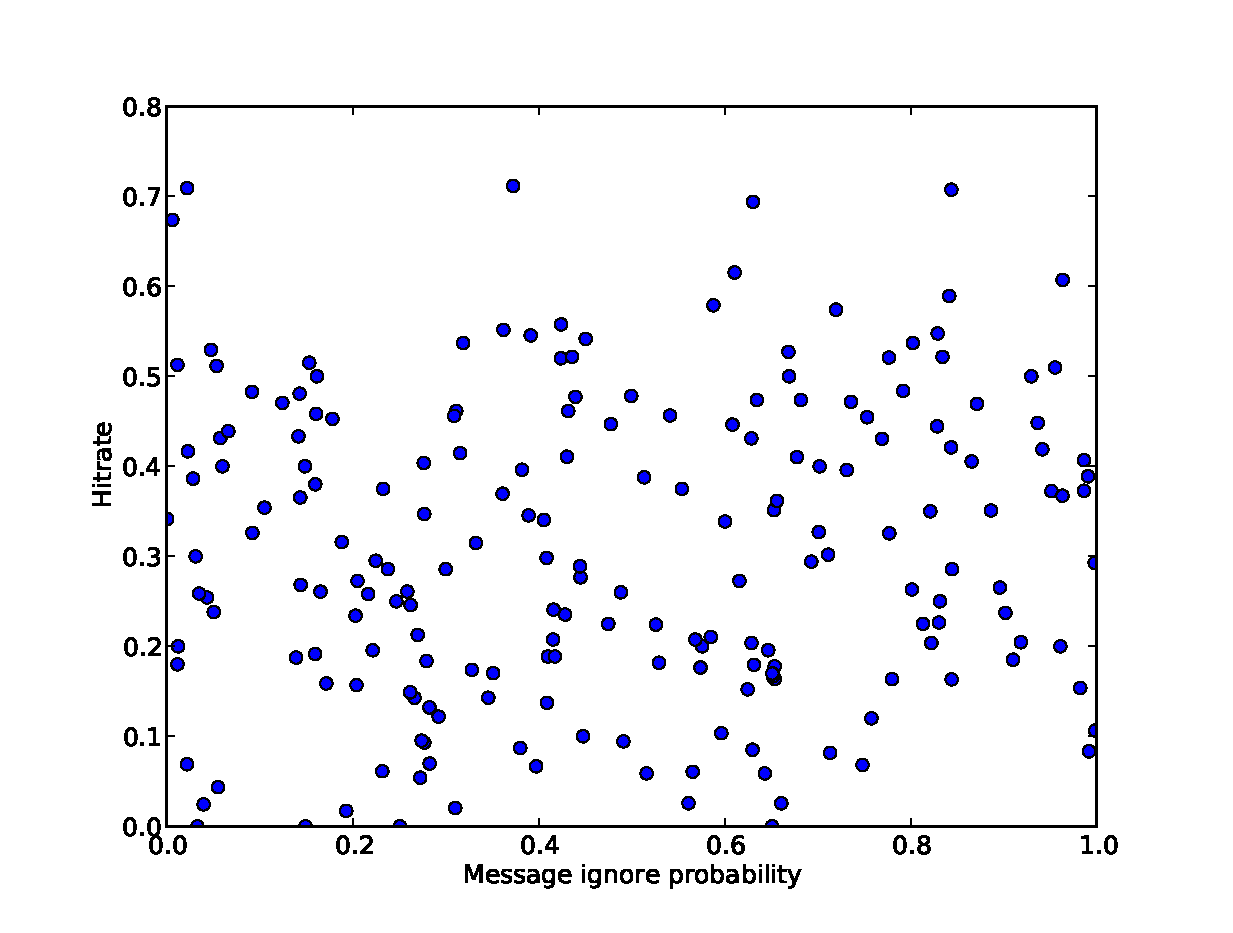
\includegraphics[width=3in]{hitrate1}
\caption{Hitrate for message ignore probability}
\label{fig:nohitrate}
\end{minipage}
\begin{minipage}[t]{3in}
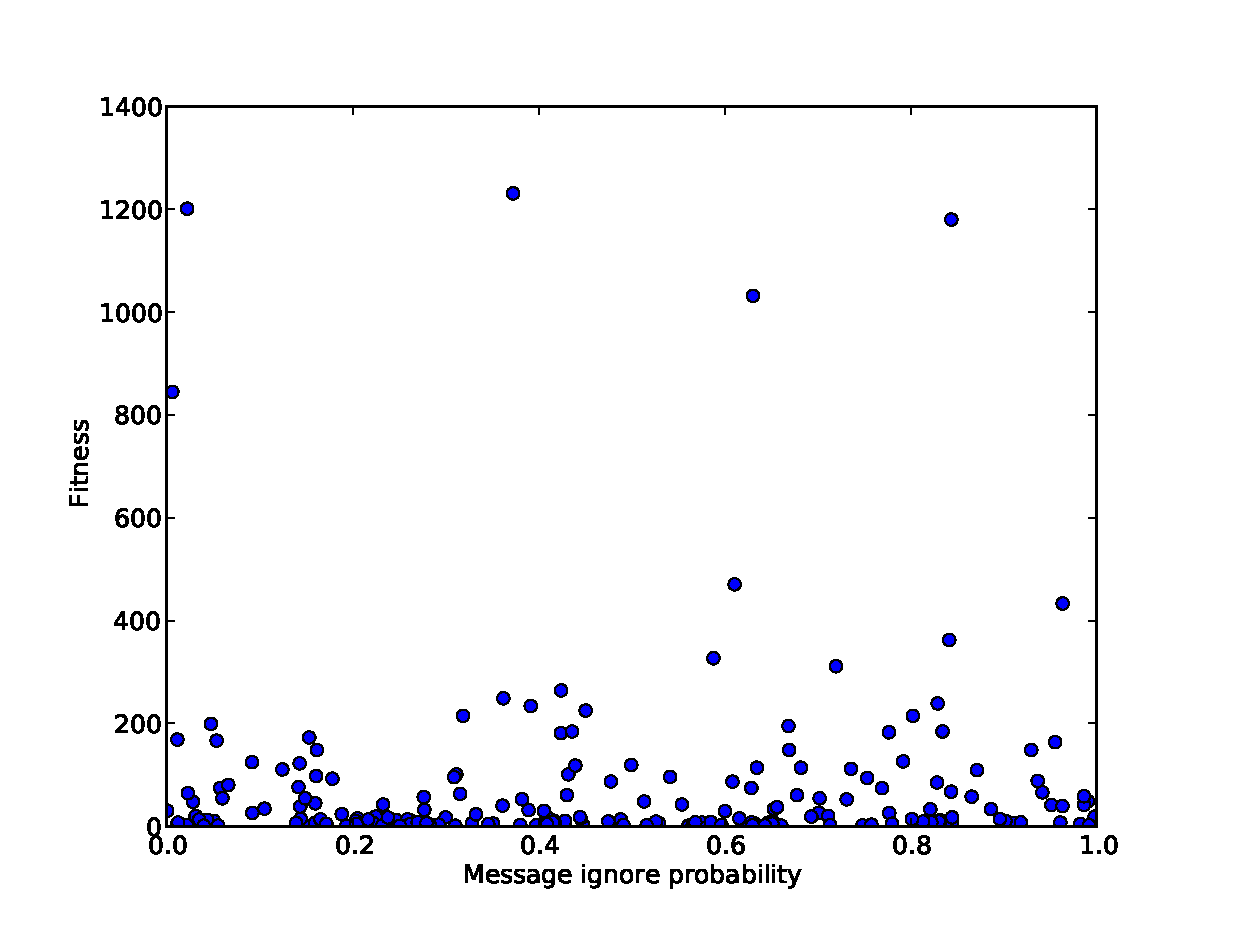
\includegraphics[width=3in]{fitness1}
\caption{Histogram of fitness for message ignore probability}
\label{fig:fitness1}
\end{minipage}
\end{tabular}
\end{figure*}

The evolution of $p_i$, hit-rate, CPU and disk cost over generations are
illustrated in Figures \ref{fig:noprob}-\ref{fig:nodisk}. 
In Figure \ref{fig:noprob}, the small group allowed to evolve independently becomes selfish, 
which means they maintain a high message ignore probability, $p_i$. This is because increasing
message ignore probability saves CPU and disk cost but does not hurt its
hit-rate.  Since the small group can evolve independently of the large group,
even if they ignore most queries, the large group will continue to answer
queries for the small group, and as such will maintain their hit-rate.

\begin{figure*}
\begin{tabular}{c c}
\begin{minipage}[t]{3in}
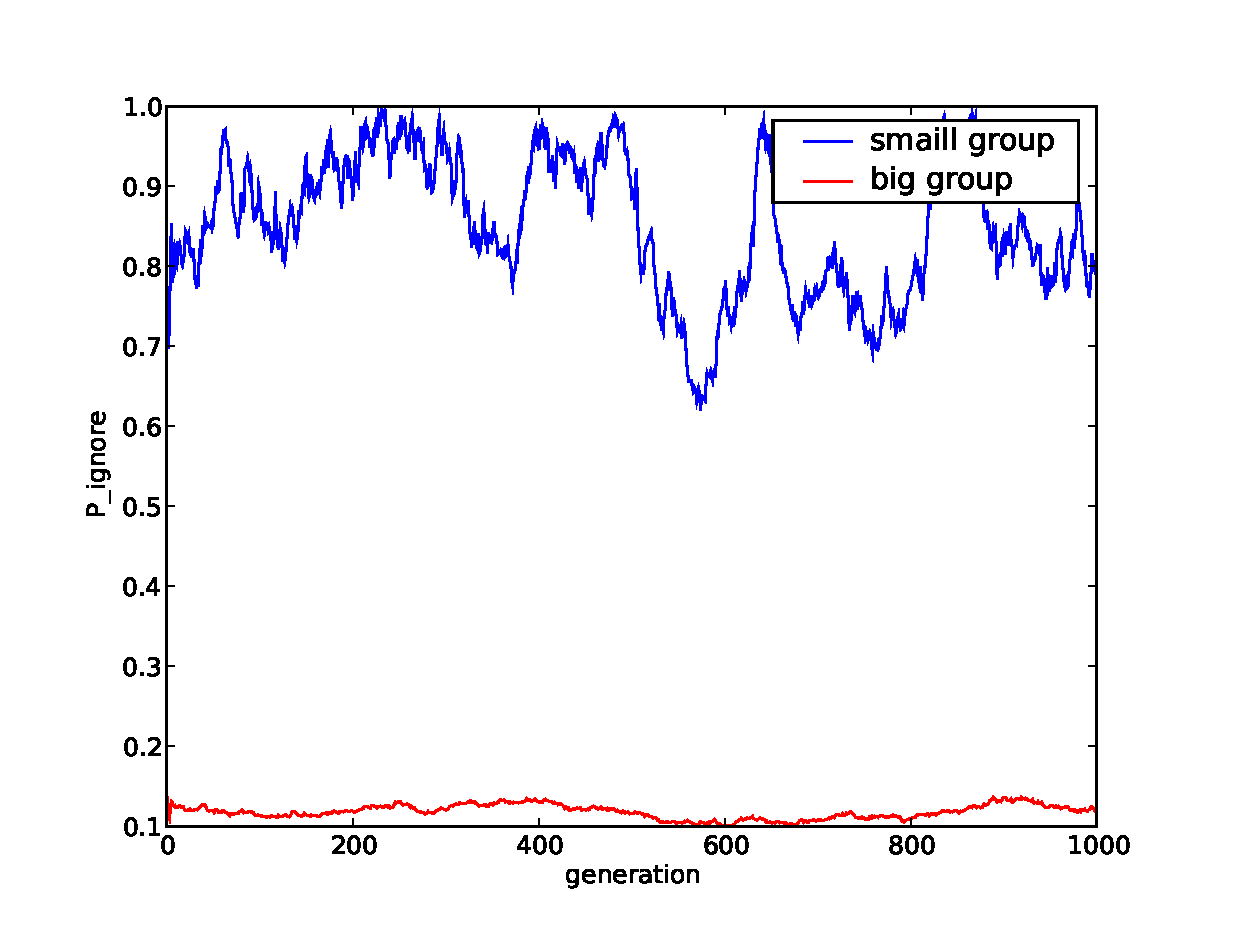
\includegraphics[width=3in]{notokenprob}
\caption{The evolution of message ignore probability without any contermeasure}
\label{fig:noprob}
\end{minipage}
&\begin{minipage}[t]{3in}
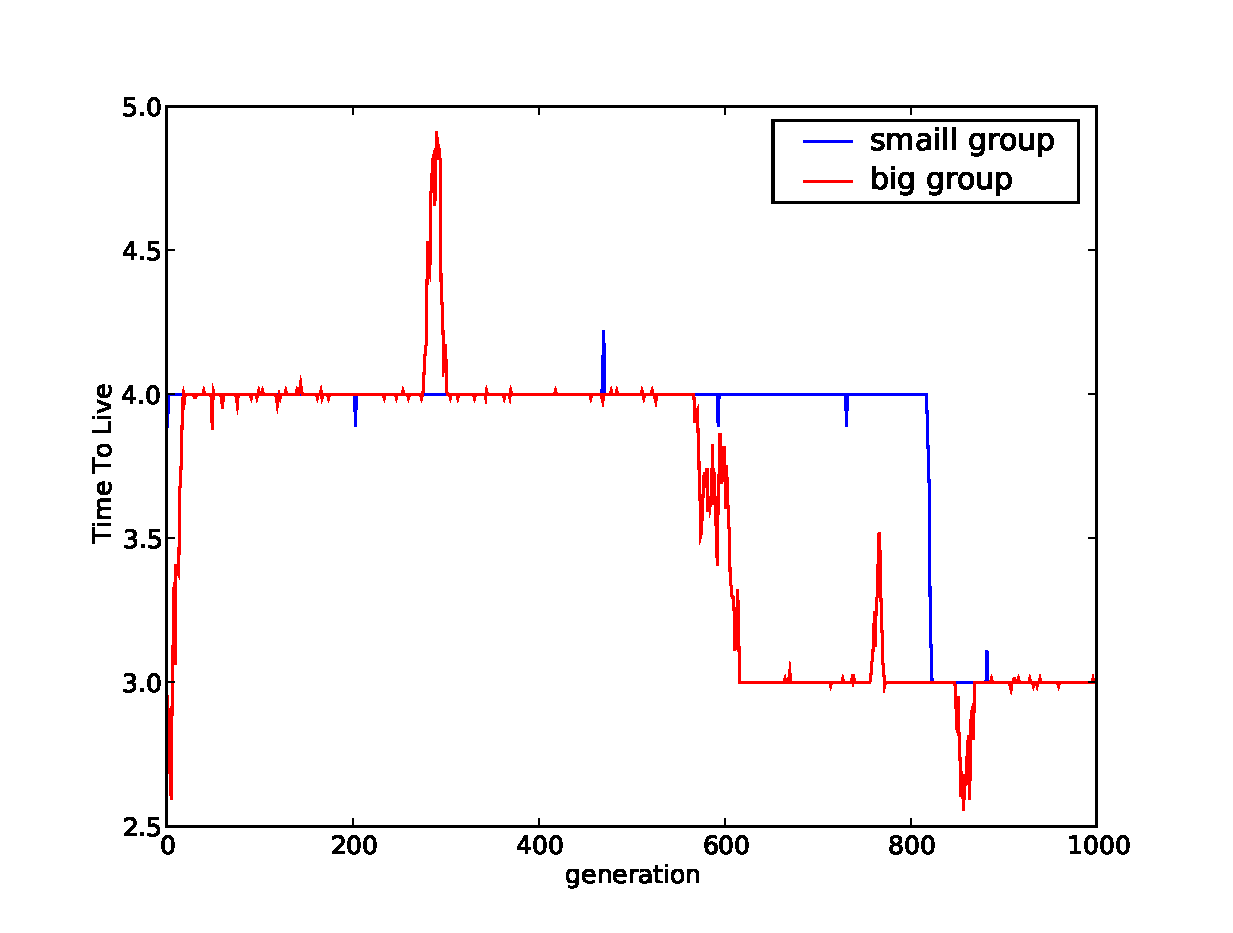
\includegraphics[width=3in]{notokenttl}
\caption{The evolution of $TTL$ without any contermeasure}
\label{fig:nottl}
\end{minipage}
\end{tabular}
\end{figure*}

\begin{figure*}
\begin{tabular}{c c}
\begin{minipage}[t]{3in}
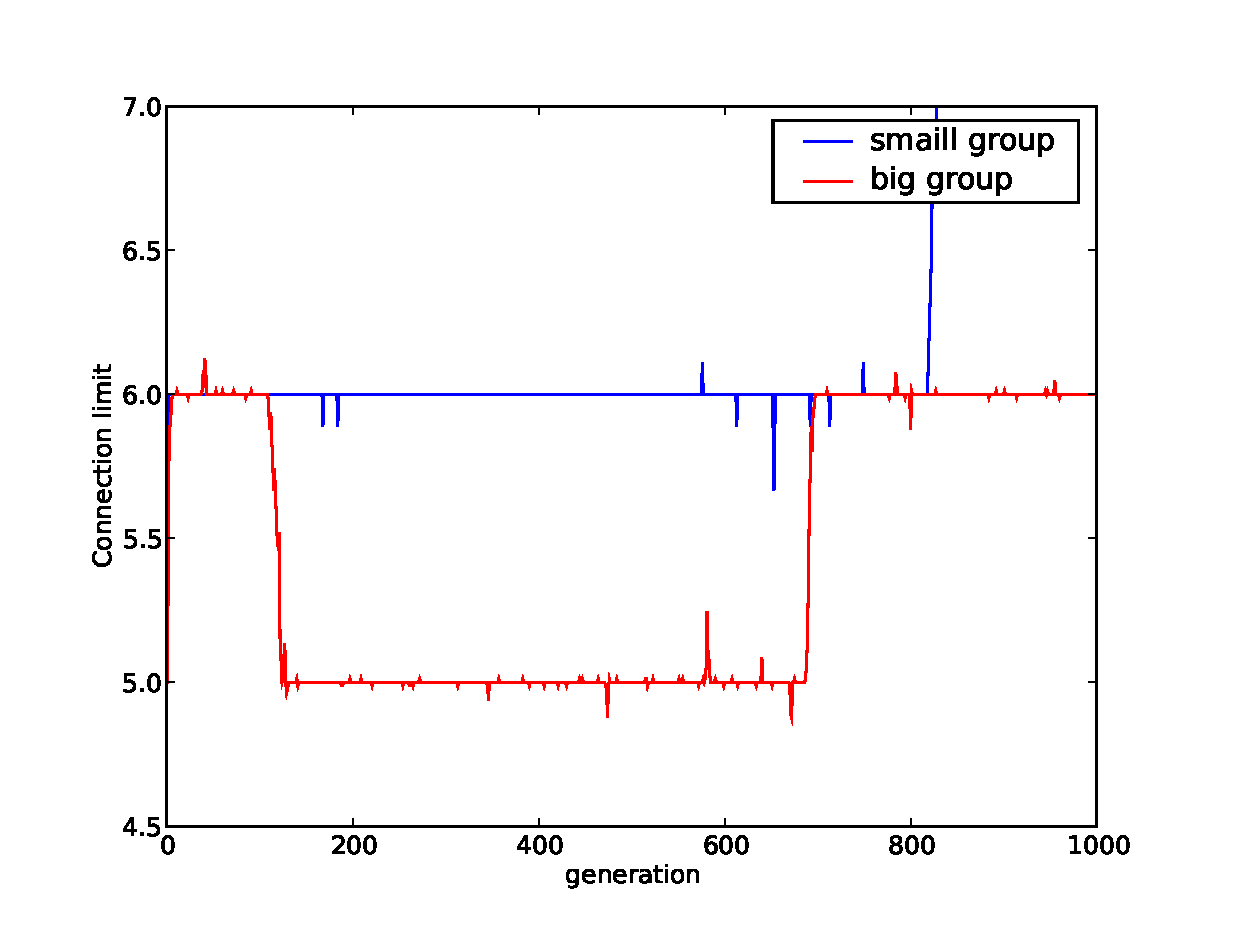
\includegraphics[width=3in]{notokenconn}
\caption{The evolution of connection limit without any countermeasure}
\label{fig:noconn}
\end{minipage}
&\begin{minipage}[t]{3in}
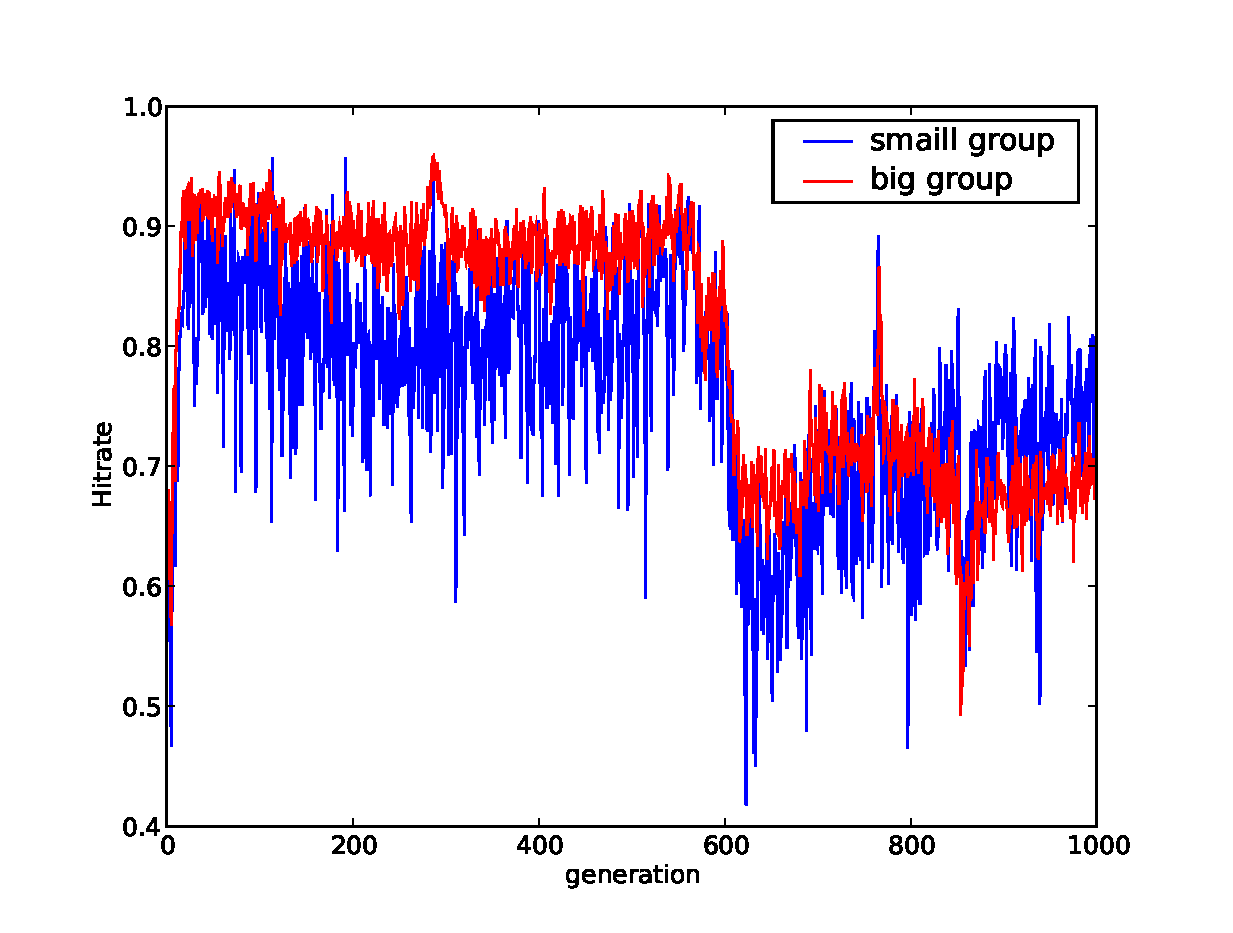
\includegraphics[width=3in]{notokenhit}
\caption{The evolution of hitrate without any countermeasure}
\label{fig:nohit}
\end{minipage}
\end{tabular}
\end{figure*}

\begin{figure*}
\begin{tabular}{c c}
\begin{minipage}[t]{3in}
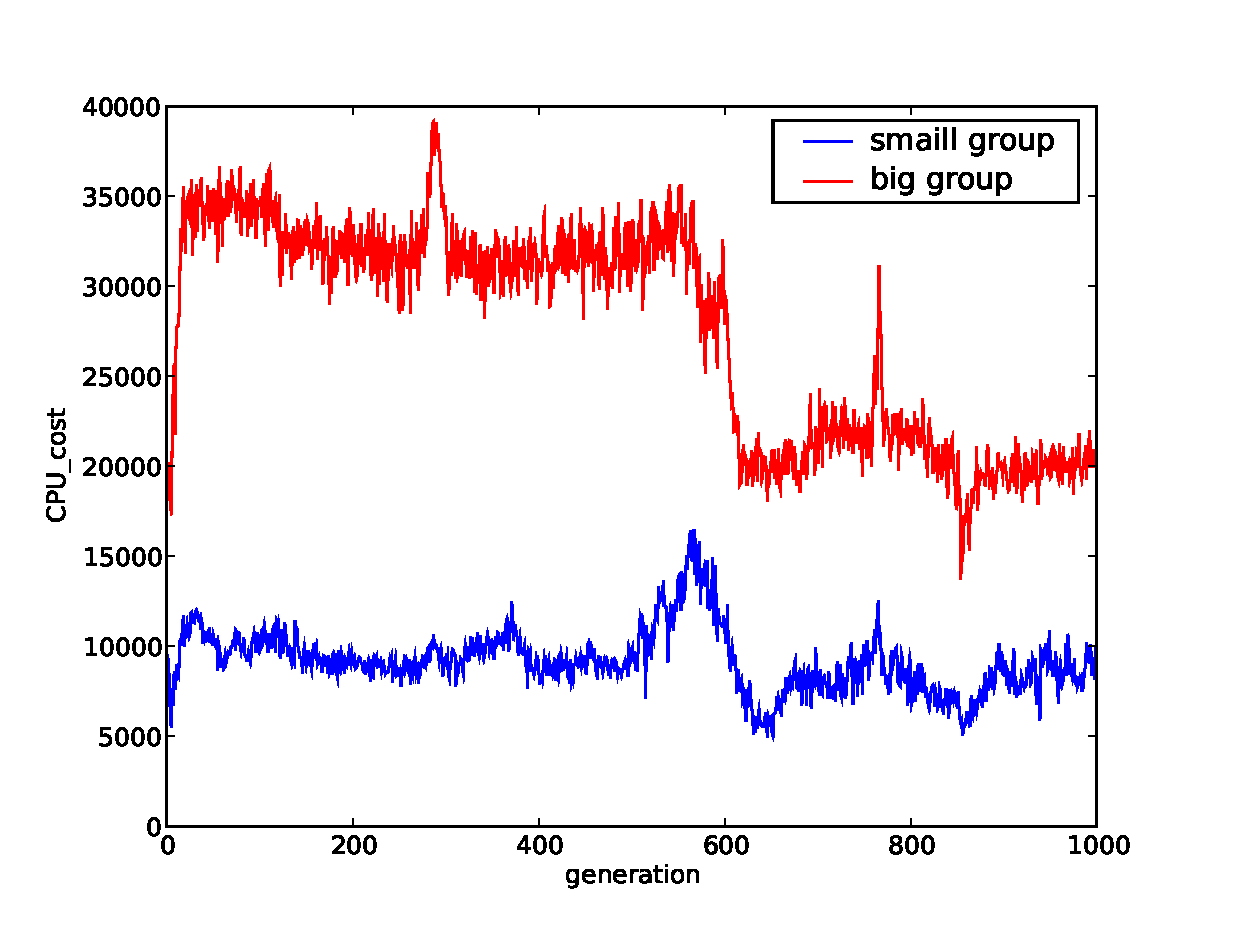
\includegraphics[width=3in]{notokencpu}
\caption{The evolution of CPU\_cost without any contermeasure}
\label{fig:nocpu}
\end{minipage}
&\begin{minipage}[t]{3in}
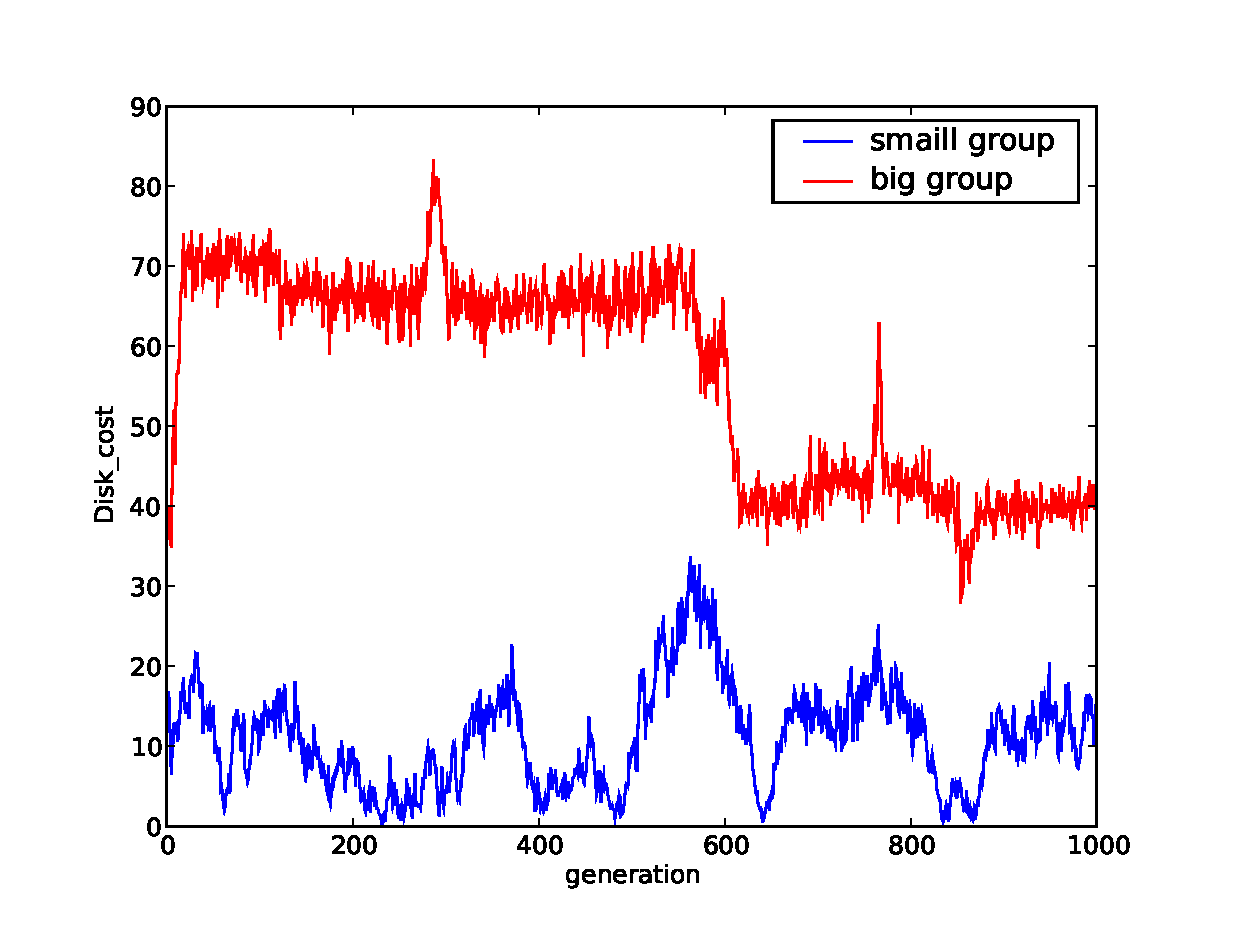
\includegraphics[width=3in]{notokendisk}
\caption{The evolution of disk\_cost without any contermeasure}
\label{fig:nodisk}
\end{minipage}
\end{tabular}
\end{figure*}

In fact, Figure \ref{fig:nohit} shows that hitrate of the small group is almost
identical to that of the big group.  The CPU and disk cost, however, is much
lower for the small group.
Around generation 600 we see a drop shift in the network.
As shown in Figure \ref{fig:nottl}, 
this is due to the big group evolving a lower $TTL$ around that time, which
has the effect of reducing the number of nodes
that see each query, reducing costs as well as slightly reducing hit-rate.

The main problem with this protocol is that a small subset of the network does
not greatly impact performance, therefore, a small subset of nodes can
free-ride.  It is undesirable to have nodes in the system consume resources
but not contribute back.  In the next section we modify the protocol to
stop this behavior.

\section{Defeating the Incentive to Free-ride}\label{sec:countermeasure}
We want each node to contribute to the performance of the network.  As we saw
in the previous section, a small isolated group tends to evolve a free-riding
strategy.
In this section we punish the hit-rate of the nodes that are ignoring
messages, (high $p_i$).
Intuitively, if we reduce the benefit that free-riders see from the network,
they should evolve a lower $p_i$ which will bring additional costs but will
on balance increase their total fitness.

\subsection{Tit-for-tat with the Reciprocal Token Method}
Node $n_A$ doesn't want to help nodes that would not help it.  To avoid doing
this, $n_A$ builds a table to track behavior.  For each node of which $n_A$ is
aware, it assigns it a token count.  If the count $n_A$ holds for a node $n_B$
is more than zero, $n_A$ will process queries from $n_B$.  Otherwise, only
with a small probabilty will $n_A$ process the message.  This small amount of
altruism is there to give a small, but non-zero, benefit to free-riders, which
makes the fitness as a function of $p_i$ less severe. 
Anytime $n_A$ receives a query response it increases the token count for the
responding node.  Anytime $n_A$ receives a query request it decreases the
token count for the requesting node.
Upon joining, $n_A$
gives each node in the network $tok_i$, so $n_A$ initially cooperates with all
nodes.  Yet, any time a node $n_B$ ignores
a query or a cache message, $n_A$ decreases the tokens it has for $n_B$.  We
encourage initial cooperation, because nodes with even a small value of $p_i$
can by chance ignore several queries, which could cause other nodes to ignore
their queries, which decreases the stability of the network.  By initially
cooperating, and cooperating in any case with a small probability, all nodes
always have an incentive to cooperate.

To help illustrate the token method, we describe three
scenarios as shown in Figure \ref{fig:token}.
The node $n_A$, sends a query which reaches $n_B$, $n_C$ and
$n_D$.  We assume $n_A$ is already aware of $n_B$ and $n_C$ but has no entry
yet for node $n_D$.  In first scenario, $n_B$ searches its neighbor token
table and serves required item if tokens for $n_A$ remain. As the consideration for $n_B$'s sharing,
$n_A$ increases the tokens for $n_B$ by one. On the other hand, $n_B$ decreases the tokens for $n_A$ by
one. Secondly, if $n_C$ ignores the query of $n_A$ or does not have the requested item, $n_A$ updates its
own neighbor token table decreasing the token for $n_C$. For last case, $n_D$
has no information about request $n_A$ nor vice-versa so $n_D$ creates the
entry for $n_A$ and initiates token value. Also node $n_A$
appends the information for $n_D$ into the neighbor token table and decreases the $n_D$'s tokens
because $n_D$ ignores the query.

In a real system, $n_A$ could test
nodes in the network by caching dummy data,
and then querying for it.  Any node in the broadcast radius that does not
send a response should have its token count decremented.  This could be done
periodically to verify that other nodes are handing caching and querying properly.

\begin{figure}
\centering
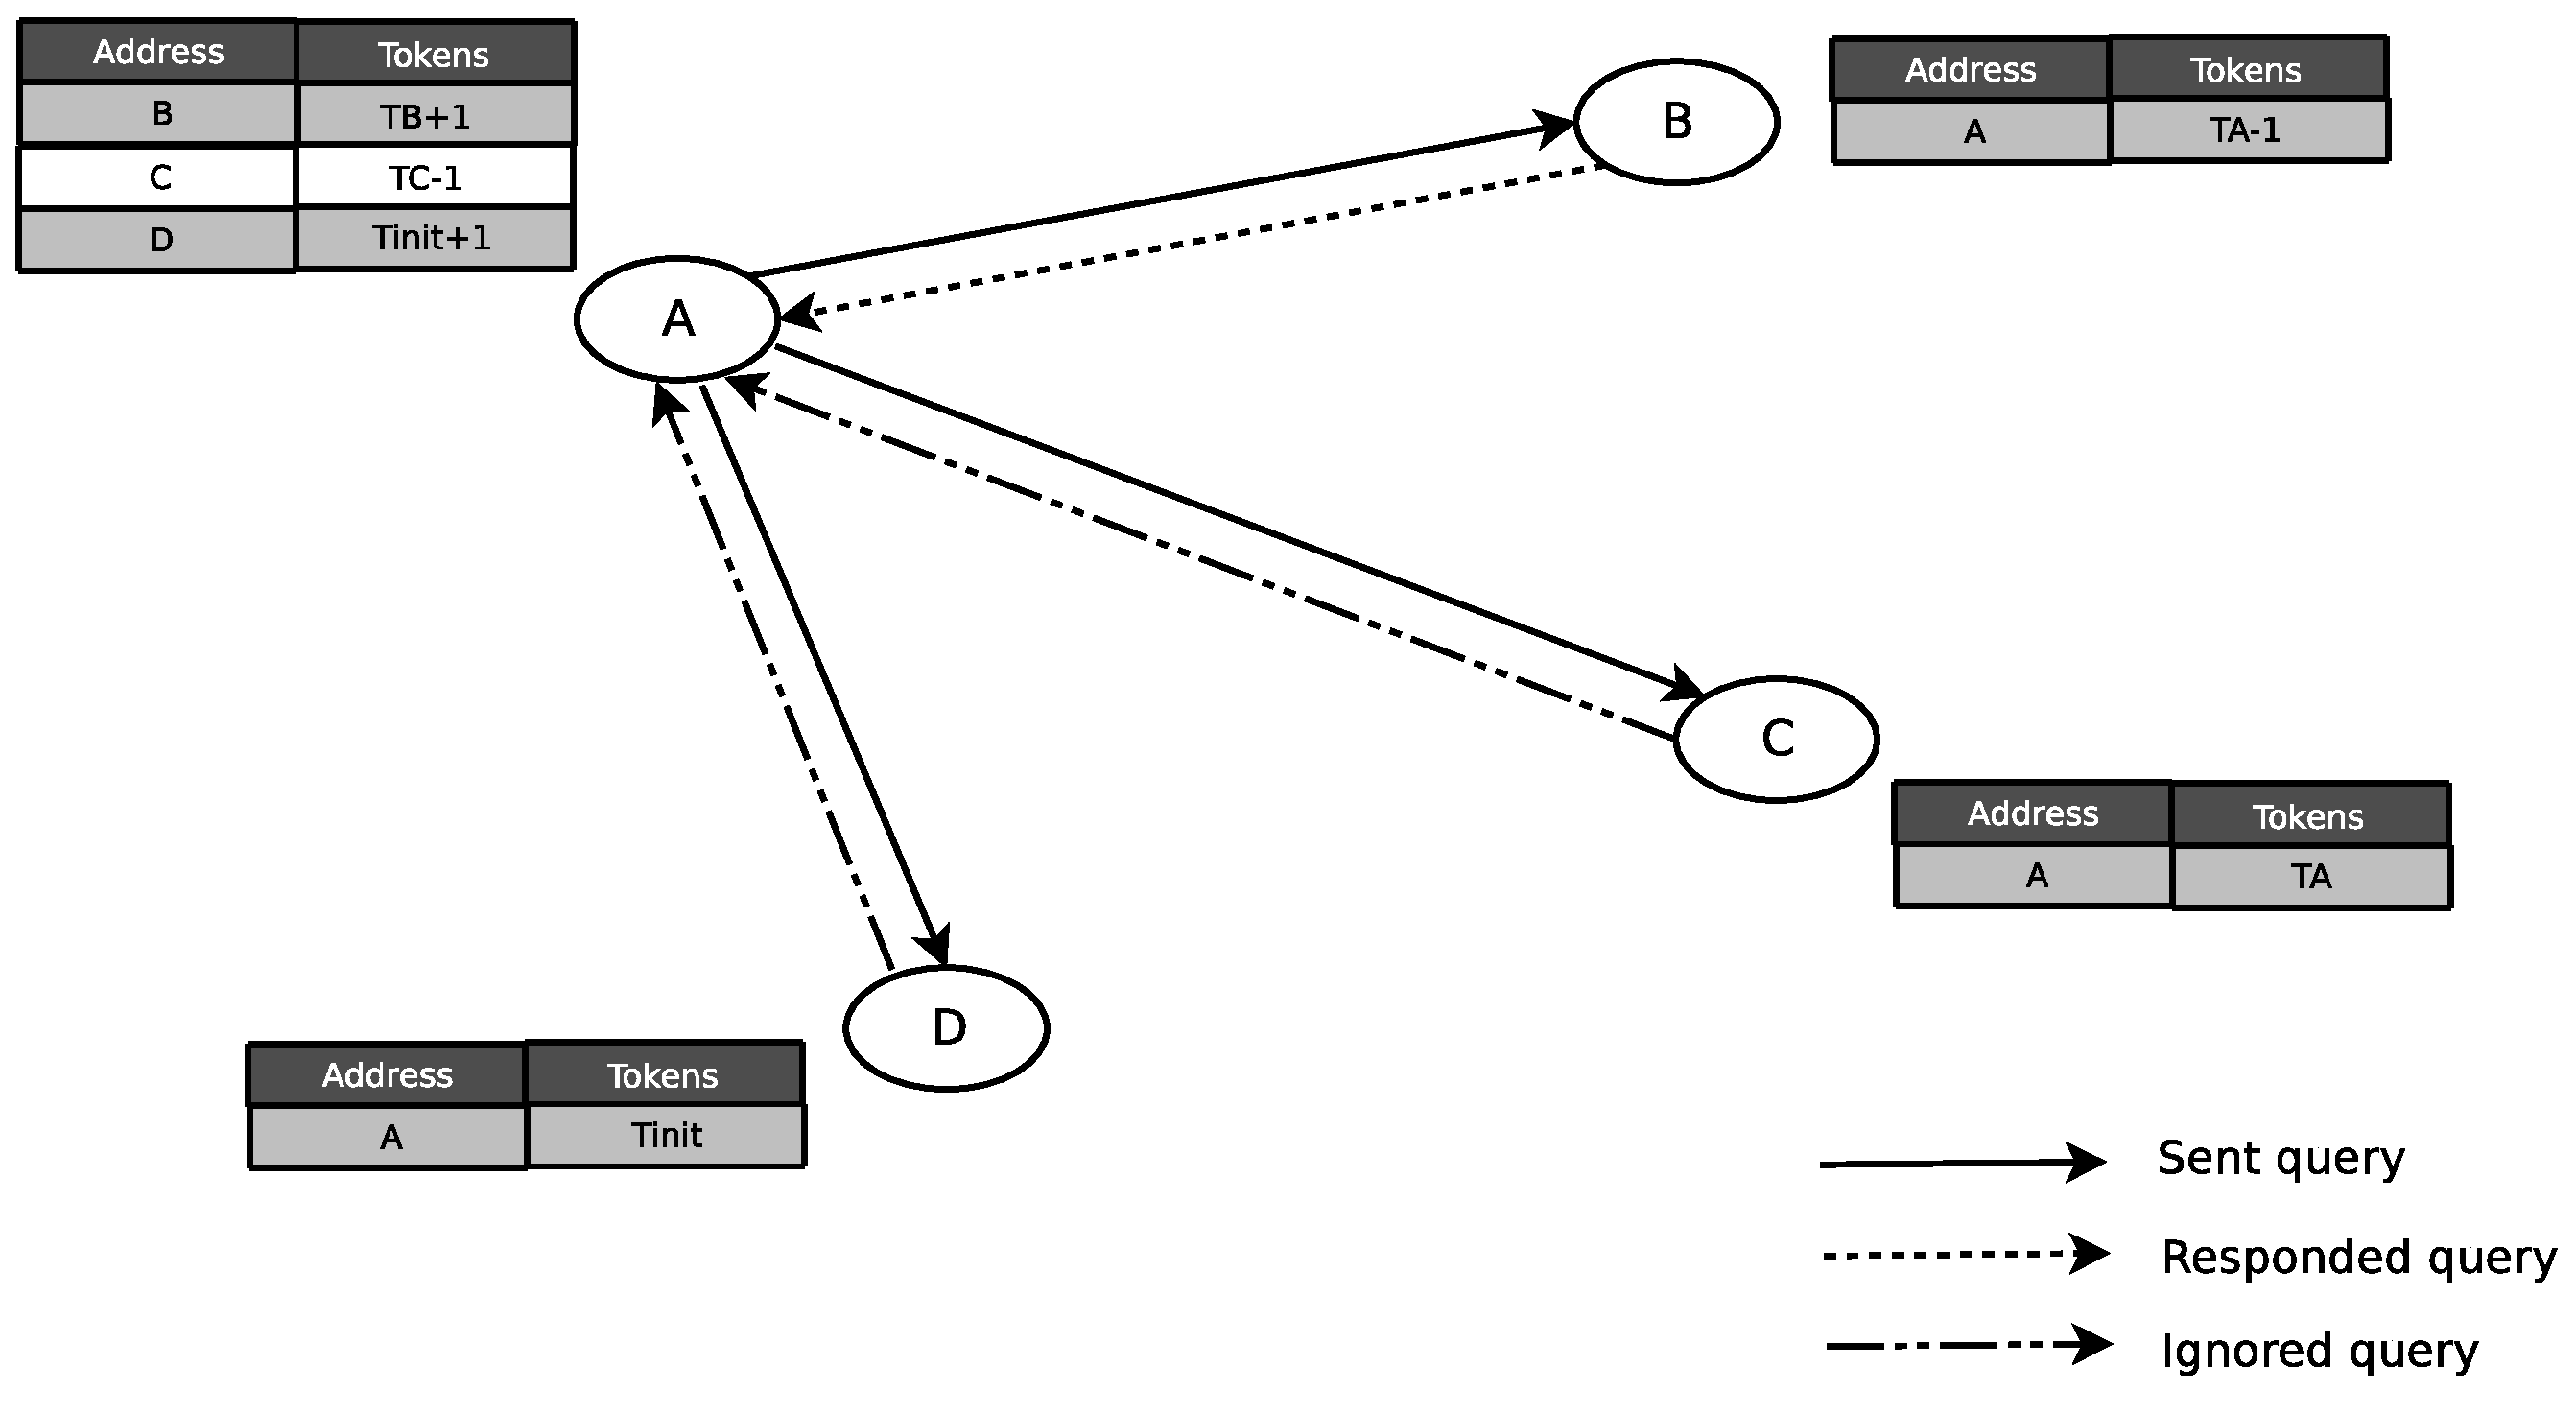
\includegraphics[width=5in]{token}
\caption{Reciprocal token method} 
\label{fig:token}
\end{figure}

In the reciprocal token method, a node which intentionally ignores the queries
of its neighbors exhaust its tokens and eventually cannot take any
benefit from the network. Ultimately, the nodes have to reduce their selfishness to get the
benefits. Our protocol is very simple, but it is enough to pressure free-riders to contribute to
the network.

Compare Figures \ref{fig:fitness1} and \ref{fig:tokenfit}.  We can
clearly see that with the reciprocal token method the fitness of nodes with
high $p_i$ is greatly reduced; moreover fitness is decreasing in $p_i$.
As such, the genetic algorithm tends to remove
such nodes from the gene pool leaving nodes with higher levels of cooperation.
In a real system, such free-riders would not benefit from ignoring queries,
and as such would either cooperate, or not participate at all.
Figures \ref{fig:tokenprob}-\ref{fig:tokendisk}
show the evolution of free riders with reciprocal token method over generations.
In Figures \ref{fig:tokenprob}
and \ref{fig:tokenhit}, see that the hit-rate of the 
small group in early generation is almost 0 due to high $p_i$.
As generations go on, however, the small group decreases its own message ignore
probability in order not to be punished and eventually behaves like big group.
Accordingly, we see hit-rate and cost go inversely with $p_i$.
As message ignore probability of small group decreases to almost the same
level as the big group, the hit-rate increases.


\begin{figure}
\centering
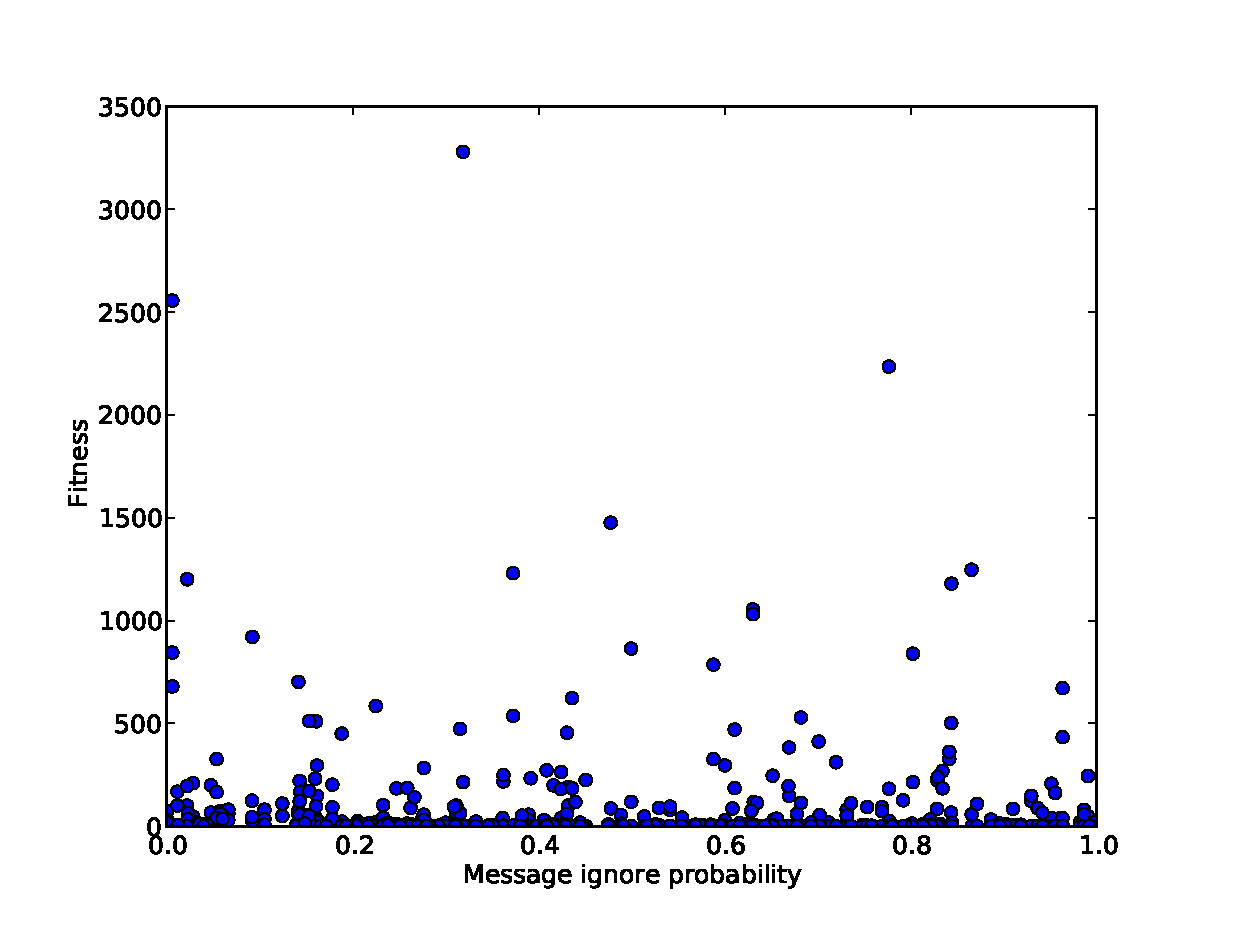
\includegraphics[width=3in]{fitness2}
\caption{Histogram of fitness for message ignore probability with reciprocal token method.
Notice that fitness decreases with selfish behavior.
}
\label{fig:tokenfit}
\end{figure}

\begin{figure*}
\begin{tabular}{c c}
\begin{minipage}[t]{3in}
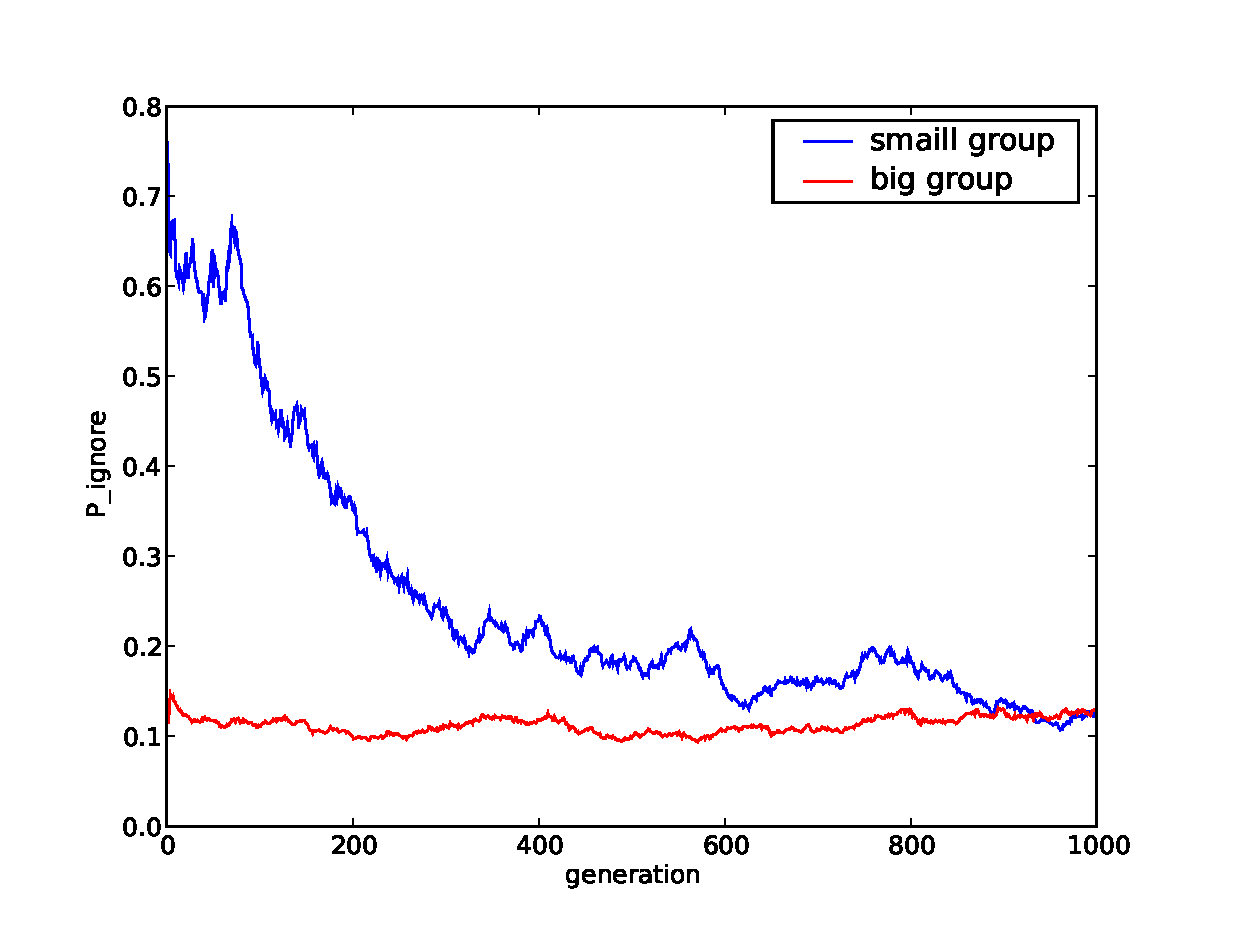
\includegraphics[width=3in]{tokenprob}
\caption{The evolution of message ignore probability with reciprocal token method as generation goes on}
\label{fig:tokenprob}
\end{minipage}
&\begin{minipage}[t]{3in}
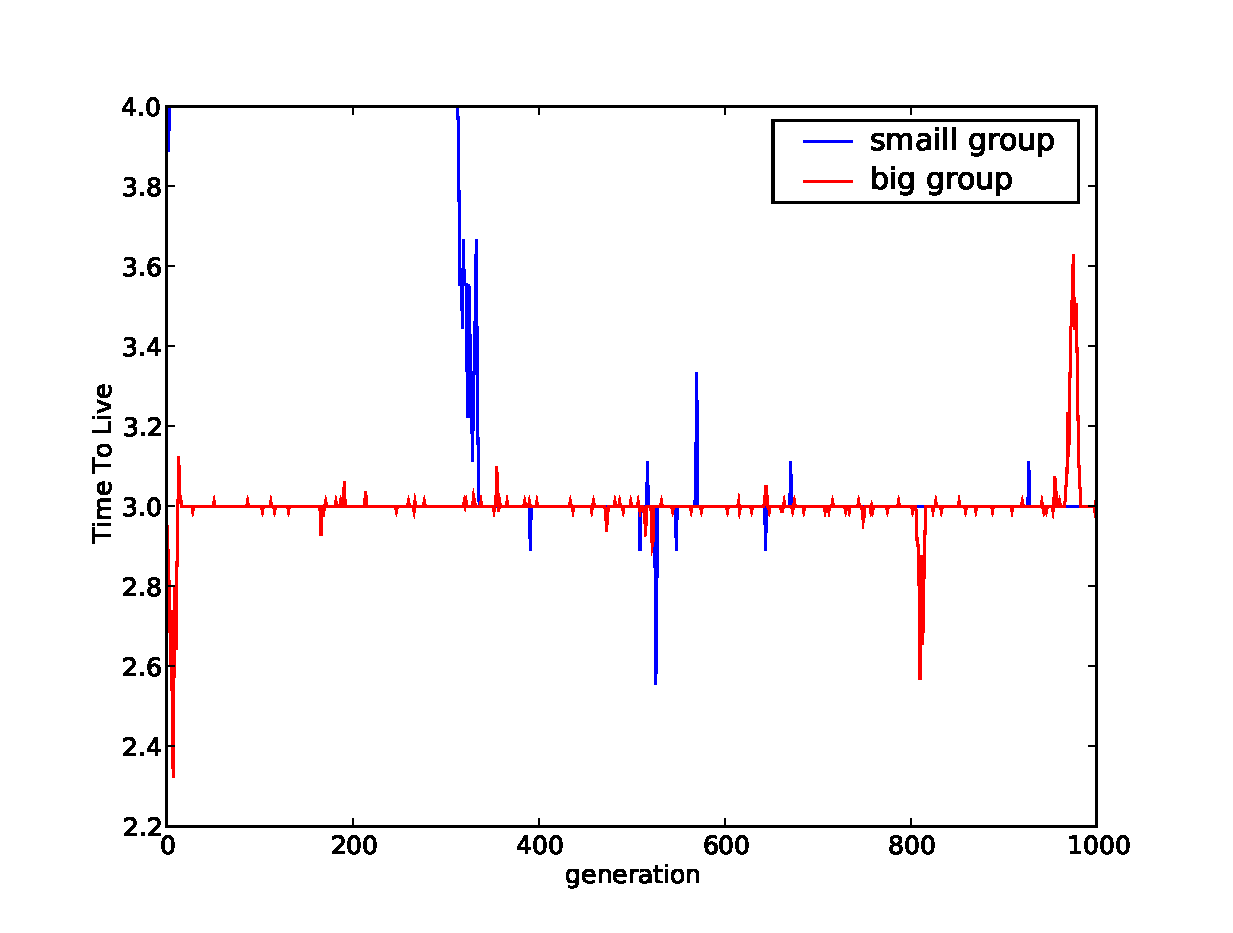
\includegraphics[width=3in]{tokenttl}
\caption{The evolution of $TTL$ with reciprocal token method as generation goes on}
\label{fig:tokenttl}
\end{minipage}
\end{tabular}
\end{figure*}

\begin{figure*}
\begin{tabular}{c c}
\begin{minipage}[t]{3in}
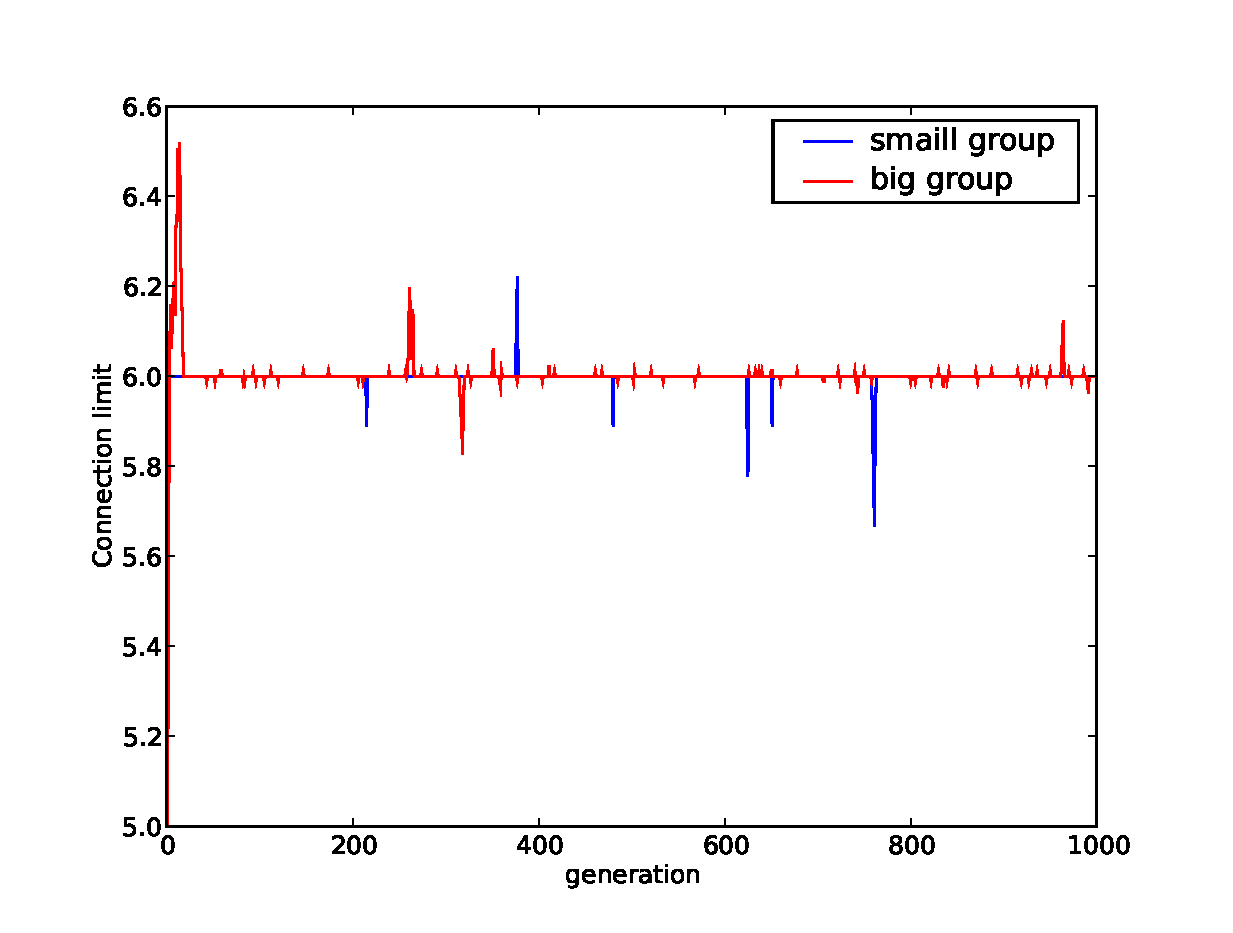
\includegraphics[width=3in]{tokenconn}
\caption{The evolution of connection limit with reciprocal token method as generation goes on}
\label{fig:tokenconn}
\end{minipage}
&\begin{minipage}[t]{3in}
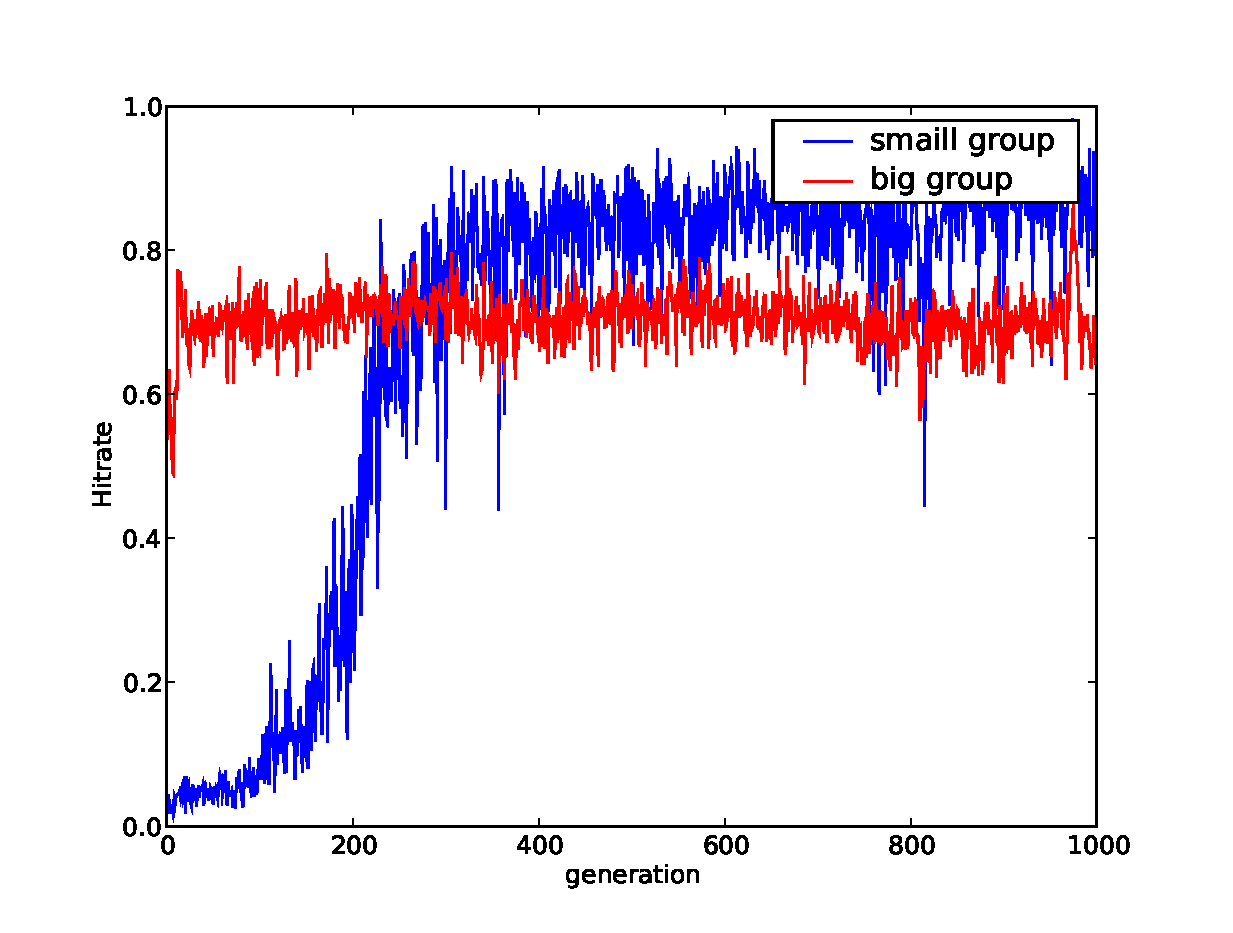
\includegraphics[width=3in]{tokenhit}
\caption{The evolution of hitrate with reciprocal token method as generation goes on}
\label{fig:tokenhit}
\end{minipage}
\end{tabular}
\end{figure*}

\begin{figure*}
\begin{tabular}{c c}
\begin{minipage}[t]{3in}
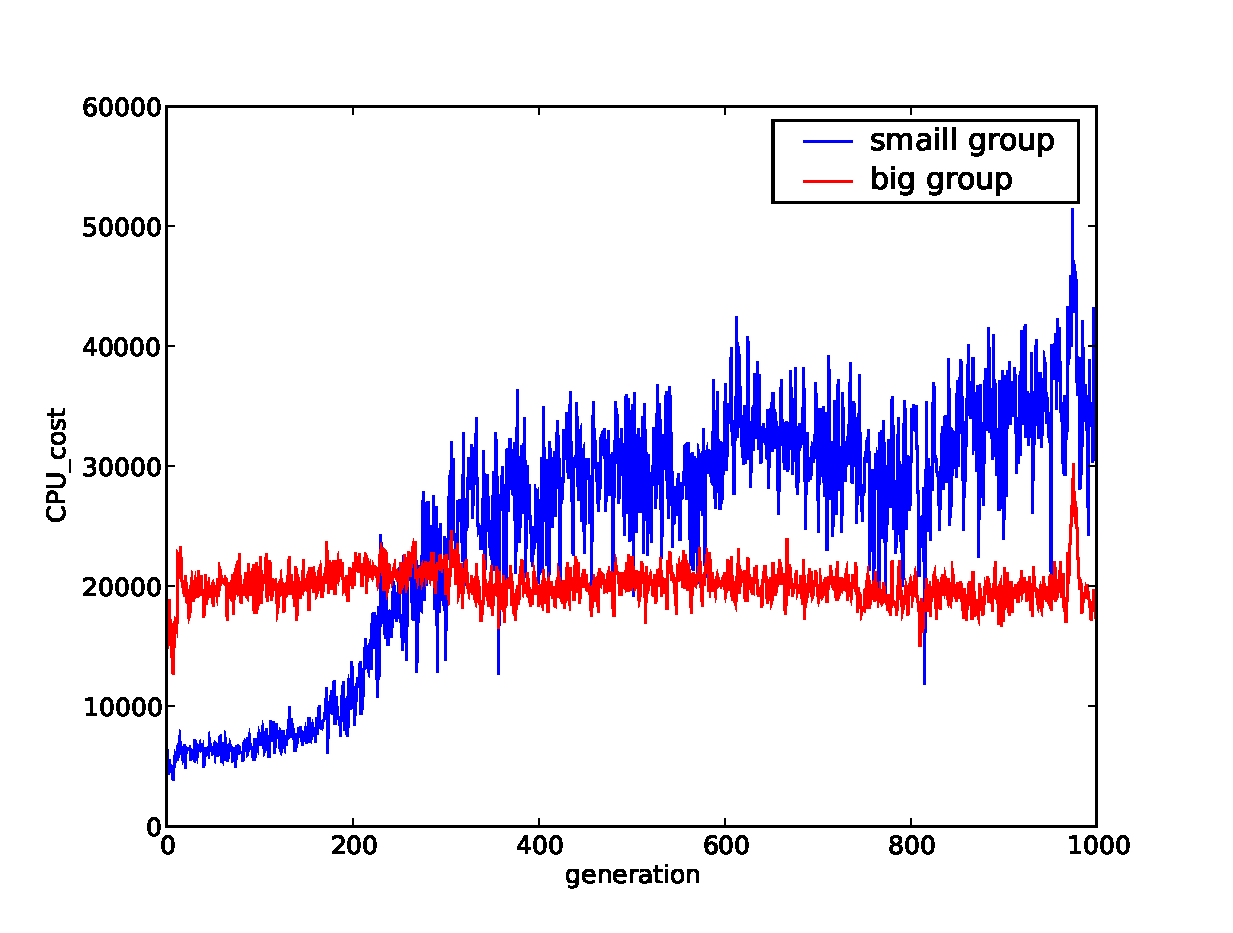
\includegraphics[width=3in]{tokencpu}
\caption{The evolution of CPU\_cost with reciprocal token method as generation goes on}
\label{fig:tokencpu}
\end{minipage}
&\begin{minipage}[t]{3in}
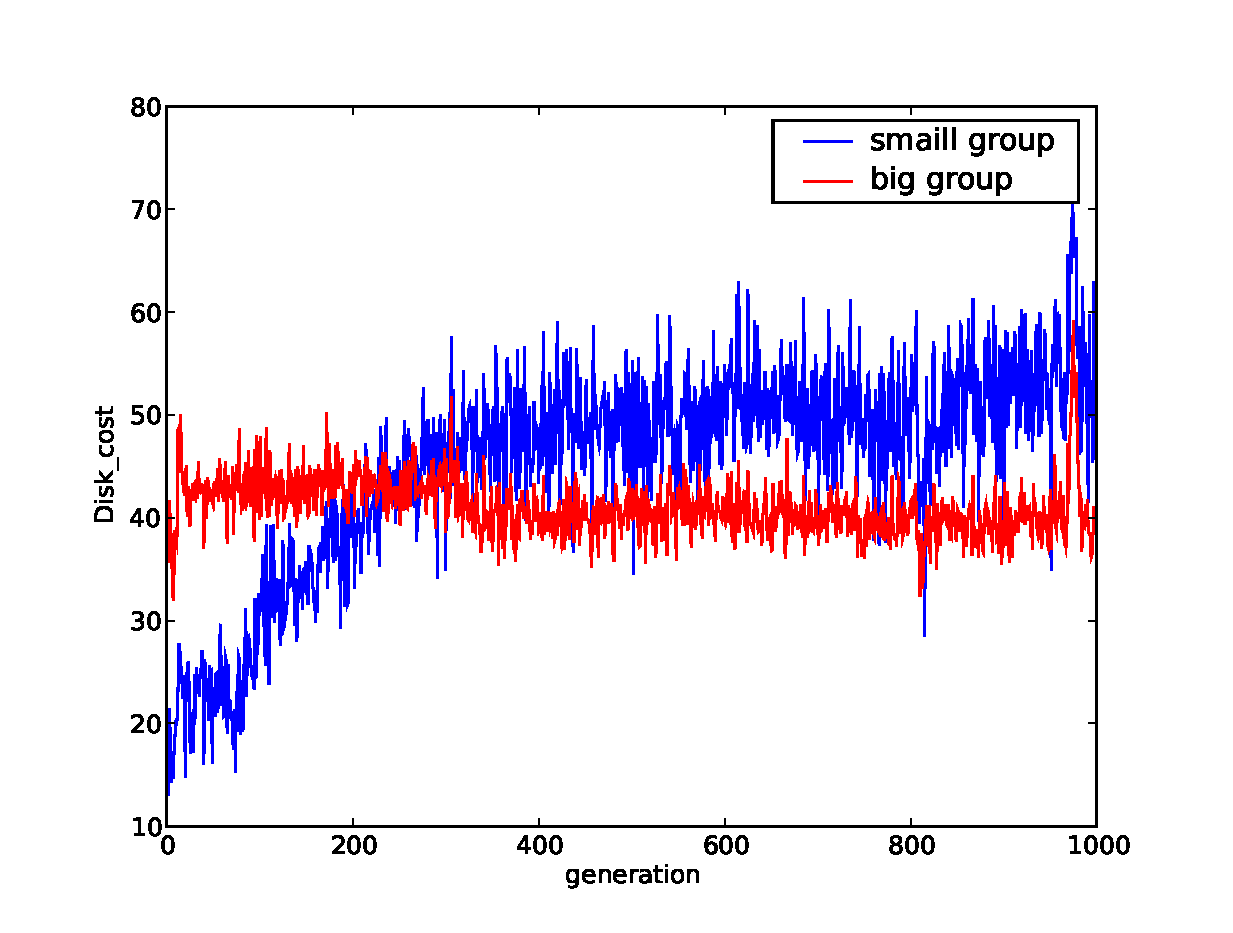
\includegraphics[width=3in]{tokendisk}
\caption{The evolution of disk\_cost with reciprocal token method as generation goes on}
\label{fig:tokendisk}
\end{minipage}
\end{tabular}
\end{figure*}

\section{Related Works}\label{sec:related}

In this paper, we show the natural evolution of free-riding by use of a genetic
algorithm. Applying the genetic algorithm to solving problems in peer-to-peer
networks has been done in various studies. One example
is the use of GAs to search optimal routing strategy for query and cache.
Firstly, to address high bandwidth consumption and poor semi-parallel search, a novel routing
function called \emph{GAroute} is proposed in \cite{conf/www/WongLK05}. In this paper,
the ID of each peer is used as a gene
and a chromosome which contains a sequence of genes represents a query routing path. In
selection process for next generation, good chromosomes with the highest information gain
and maximum length are primarily selected. Iles et al.\cite{Iles02} search for
routing strategies in P2P networks using genetic programming. In this study, results
from simulation on P2P networks are described in which genetic programming is used
to evolve routing strategies that optimize resource location in various traffic low scenarios.
The network protocol consists of two expressions: the CONN expression which
specifies the
number of connection to be maintained, and the RANK expression which is used to rank the
connections. Each expression are represented as trees and manipulated using crossover and
mutation operations.
Koo et al.\cite{journals/fgcs/KooKL06} propose a genetic algorithm based on 
neighbor selection strategies which are
incentive-compatible and suitable for real time deployment for P2P networks.
Furthermore, the strategy proposed by that study has been compared with the existing
strategy using two welfare metrics: system throughput and average downloading time.
In \cite{IIHMSP07}, a genetic algorithm is combined with ant routing.
A GA is used to find the coarsest \emph{GridPeer} resources.  Then, the result
is refined using into an ant algorithm, this combination gives more
accurate resources discovery than either alone.

The crucial difference between above works and our study is what role the GA
plays in improving system design. While previous studies we mentioned in this section use the
genetic algorithm as solution to search for optimal value for problems they
define where there is generally a global definition of fitness to find a
single protocol for each node to follow, we use the GA to allow each node to
effectively compete against each other to evolve strategies to minimize their
costs and maximize their benefits.  Our work is applicable to many P2P systems
where the communication protocol allows sufficient flexibility for nodes to
follow different local algorithms while still communicating with each other.
 
\section{Conclusion and Future works}\label{sec:concl}

Contrary to some prior works, we used a genetic algorithm to find
\emph{locally rather than globally optimal behavior}.
We show that even with a very simple flooding protocol, free-riding naturally
evolves and degrades network performance.
In addition, we proposed a tit-for-tat solution to prevent free-riders
from behaving selfishly and
ultimately induce them to contribute to the network.

In this work, we focused on nodes ignoring messages.  Nodes can also
selfishly choose very large TTL values which cost the network more to process
requests, since they reach more nodes, but may not significantly increase
hit-rates.  Additionally, cheating strategies could be expanded beyond simply
ignoring messages.
For future work, we will model a richer protocol with a richer set of
behaviors.  A more powerful approach is to model all the allowed behaviors
with a genetic program.  Each node can evolve its own algorithm for each part
of the network: joining, querying, caching, and routing.
Using a genetic programming paradigm, we expect more complex tit-for-tat
strategies to naturally evolve.
A problem we would like to address is how to create protocols that force each
local node into a behavior which optimizes the fitness of the entire network,
or put another way, how do we build a protocol such that selfishly looking out
for one's own interest is the best thing a node can do for the entire network.

\bibliographystyle{IEEEtran}
\bibliography{genetic}

\end{document}

]
